\documentclass[a4paper, 15pt]{article}
\usepackage[T1]{fontenc}
\usepackage[utf8]{inputenc}
\usepackage[italian]{babel}
\usepackage[none]{hyphenat} % no sillabazione 

\usepackage{multicol} %testo su più colonne
\usepackage{enumerate}
\usepackage{mdwlist} %suspend enumerate \suspend{} \resume{}
\usepackage{lipsum} %testo random per verifica \lipsum
\usepackage{graphicx, nicefrac}
\graphicspath{{figures/}} % Directory in which figures are stored
\usepackage{wrapfig2}
\usepackage{amsmath}
\usepackage{amssymb}
\usepackage{amsthm} %teoremi e dimostrazioni e definizioni
\usepackage{cases}
\usepackage{gensymb} %simboli come ° = \degree  etc etc
\usepackage{cancel} %permette di fare semplificazioni utilizzando il comando \cancel{expression}
\usepackage{subcaption}
\usepackage{hyperref}
\hypersetup{
	colorlinks=true,
	linkcolor=blue,    
	urlcolor=blue,
	%pdfpagemode=FullScreen, %il pdf generato non si avvia a schermo intero
}
\urlstyle{same}
\usepackage{changepage}
\usepackage{lastpage, epstopdf}
\usepackage{fancyhdr}
\usepackage{tcolorbox}
%\usepackage{background} %non utilizza lo sfondo con "draft"
\usepackage{color} % testo colorato \textcolor{'ColorCode'}{'testo'}
\usepackage{setspace} % in questo modo posso settare lo spoazio dell'indice
\raggedbottom
\setlength{\parindent}{0pt}
%========TEOREMI========%
\newtheorem*{thm}{Teorema}
\newtheorem*{en}{Enunciato}
\newtheorem*{definizione}{Definizione}
\newtheorem*{cor}{Corollario}



%========OPERATORI========%
\DeclareMathOperator{\rk}{rk}
\DeclareMathOperator{\im}{Im}

\newcommand{\compresslist}{ % Define a command to reduce spacing within itemize/enumerate environments, this is used right after \begin{itemize} or \begin{enumerate}
			\setlength{\itemsep}{1pt}
			\setlength{\parskip}{0pt}
			\setlength{\parsep}{0pt}
		}

\title{Alcuni appunti di \\
	 Tecnologie Meccaniche\\ {\small A.A. 2022-2023}}
%\author{A.M.}
\date{}

\begin{document}
	
	\maketitle
	\setcounterpageref{secnumdepth}{0}
	
	\begin{spacing}{0.85} % In questo modo setto lo spazio dell'indice
		\tableofcontents
	\end{spacing}
	\newpage
	
	\part{Deformazione Plastica}
	
	Nelle deformazioni plastiche gli atomi del materiale passano per successive posizioni di equilibrio: il volume si conserva. \\
	
	Si deformano meglio i materiali che vengono dal processo fusorio in forma transitoria, posseggono infatti grani più grossi e le dislocazioni possono viaggiare di più. \\
	
	La configurazione CFC si presta meglio alla deformazione plastica, sebbene abbia solo 12 piani di scorrimento ha un alto valore di $a$ e quindi un basso valore di $\tau$.
	\begin{center}		
		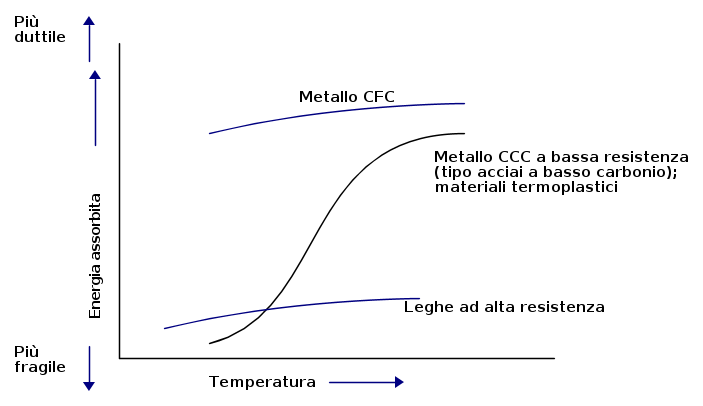
\includegraphics[width=0.8\linewidth]{def1}		
	\end{center}
	La tensione tangenziale massima è proporzionale 
\begin{equation}\label{eq:1}
	\tau_{\max}\propto{b\over a}
\end{equation}
	In cui $a$ è il parametro di cella e $b$ è la densità atomica sul piano di scorrimento. 
	
	Un materiale CCC nonostante abbia 48 piani di scorrimento,  $a\downarrow$ e $\tau\uparrow$, lavorando a caldo si aumenta la mobilità atomica e $a\uparrow \tau\downarrow$.
\newpage	
	\section{Temperatura e Velocità}
	All'aumentare della temperatura aumenta la mobilità atomica, questo significa avere celle di più grandi dimensioni: $a\uparrow~\Rightarrow~\tau\downarrow$
	
	Lavorando a caldo, a $\theta= {2\over3}$ si aumenta la velocità di ricristallizzazione piuttosto che quella di incrudimento e si aumenta la produttività ma si incorre nel rischio di ossidazione e non si hanno miglioramenti delle caratteristiche meccaniche.\\
	
	A maggiori velocità di applicazione del carico il materiale risponde con un comportamento più rigido. 
	
	Anche questo fattore è influenzato dalla temperatura: come questa aumenta, cresce l'inerzia degli atomi a muoversi contemporaneamente nella stessa direzione, aumenteranno di conseguenza le tensioni da fornire per portare a termine la lavorazione. 	
\begin{center}
	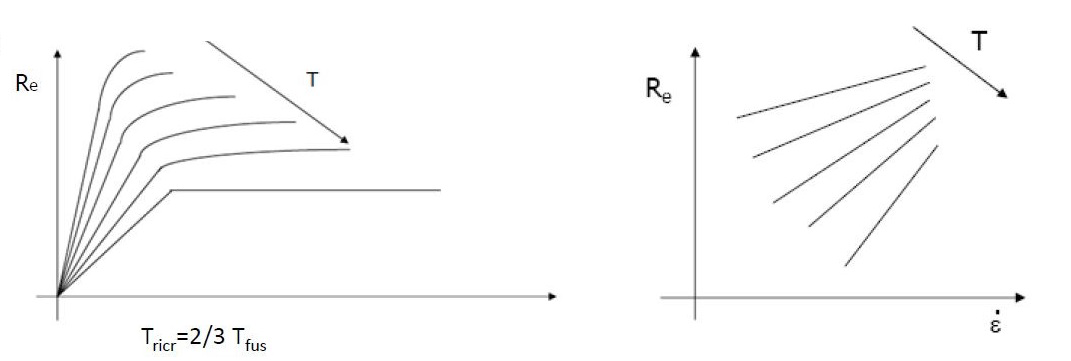
\includegraphics[width=0.8\linewidth]{figures/def2}
\end{center}
	 \section{Legame sforzo - deformazione}
	 La deformazione plastica avviene tridimensionalmente, ma le prove di caratterizzazione dei materiali sono monoassiali. 
	 
	 Si ricorre al criterio di Von Mises per la determinazione di uno stato equivalente monoassiale. \\
	 
	 Viene raggiunto lo snervamento quando la relazione tra le tensioni principali e la tensione di snervamento vale
	 \[(\sigma_1-\sigma_2)^2+(\sigma_2-\sigma_3)^2+(\sigma_3-\sigma_1)^2 = 2\sigma_Y\]
	 Quando le tensioni sono sufficientemente elevate e causano deformazioni plastiche, le relazioni tra tensioni e deformazioni sono ottenute dalle equazioni di Levy-Mises
	 \[\dfrac{d\varepsilon_1}{dt}\dfrac{1}{\sigma_1'} = \dfrac{d\varepsilon_2}{dt}\dfrac{1}{\sigma_2'} = \dfrac{d\varepsilon_3}{dt}\dfrac{1}{\sigma_3'}\]
	 In cui 
	 \[\sigma_i'= \sigma_1 - {1\over3}(\sigma_1+\sigma_2+\sigma_3) = \sigma_1 - {1\over2}(\sigma_2-\sigma_3)\]
	 Allora 
	 \[\dfrac{d\varepsilon_1}{dt}\dfrac{1}{\sigma_1'} = \dfrac{\dot{\varepsilon}}{\sigma_1 - {1\over2}(\sigma_2-\sigma_3)}\]
	 
	 In caso di \textbf{deformazione piana} si ponga essere $\varepsilon_2=0 \Rightarrow\dot{\varepsilon_2}=0$, allora per fare in modo che le equazioni di Levy-Mises rimangano non nulle deve essere 
	 \[\sigma_2 = {1\over2}(\sigma_2+\sigma_3)\]
	 Che sostituita all'interno dell'equazione di Von Mises porta a 
	 \begin{equation}\label{eq:VM}
	 	\boxed{(\sigma_1-\sigma_3)^2 = {4\over3}\sigma^2_Y}
	 \end{equation}
	 Condizione di plasticità di Von Mises.\\
	 
	 In caso di \textbf{tensione piana} si sostituisce semplicemente ad esempio $\sigma_2 = 0$ all'interno dell'equazione di Von Mises e si ottiene
	 \[\sigma_1^2+\sigma_3^2-\sigma_3\sigma_1 = \sigma_Y^2\]
	 
	 Il concetto principale è che si ha sempre una direzione preponderante per la quale la forza d'attrito è maggiore. 
	 
	 \section{Slab Method}
	 Metodo semplificato che permette di calcolare la forze di chiusura di uno stampo imponendo l'equilibrio su un parallelepipedo infinitesimo di materiale sottoposto a deformazione. 
	 
	 Le ipotesi da verifica per applicare lo Slab Method sono
	 \begin{itemize}\compresslist
	 	\item \textbf{Stato deformativo piano}: esistenza di una dimensione predominante rispetto alle altre. Generalmente verificata
	 	\item \textbf{Materiale isotropo}: policristallino, senza tessiture, plastico secondo Von MIses. Generalmente verificata
	 	\item \textbf{Assenza di Barreling}: le superfici laterali piane devono restare piane anche dopo la deformazione> Ipotesi meno verificata
	 \end{itemize}
 	\subsection{Stampaggio - Fucinatura}
 	In uno stampo la profondità è molto minore della lunghezza: c'è una dimensione principale sulla quale agiscono le forze di attrito, lo stato deformativo è piano. 
\begin{center}
	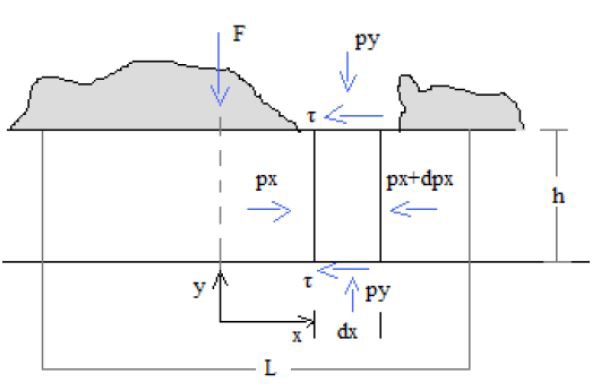
\includegraphics[width=0.5\linewidth]{figures/def3}
\end{center}
	 L'equilibrio delle forze lungo $x$ vale
	 \[P_xhb - (P_x+dP_x)hb - 2\cdot\tau dxb = 0 \Rightarrow \cancel{P_xhb} - \cancel{P_xhb} - dP_xhb - 2\tau dxb = 0 \Rightarrow dP_xh = -2\tau dx \Rightarrow \dfrac{dP_x}{dx} = -2{\tau\over h} \]
	 \begin{equation}\label{eq:5}
	 	\dfrac{dP_x}{dx} = -2{\tau\over h}
	 \end{equation}
	 Applicando la condizione di plasticità di Von Misese si ottiene
	 \[\sigma_1-\sigma_2 = \pm{2\over\sqrt{3}}\sigma_0\]
\begin{center}
	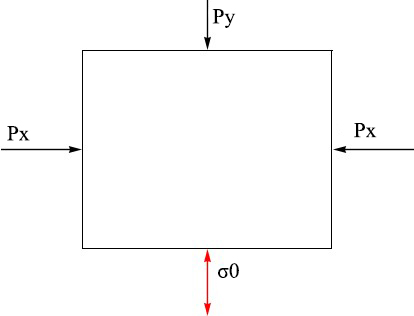
\includegraphics[width=0.5\linewidth]{figures/def4.0}
\end{center}	 
	 Sotto le ipotesi che 1 e 2 siano direzioni principali e combacino rispettivamente con $x$ e $y$, si può scrivere, dato che sono entrambi sforzi di compressione:
	 \[\sigma_1 = -P_x\qquad\sigma_2=-P_y\]
	 Allora
	\[-P_x-(-P_y) = \pm{2\over\sqrt{3}}\sigma_0\]
	\[-P_x+P_y = \pm{2\over\sqrt{3}}\sigma_0\]
	Ad $x = L/a, P_x = 0$ il corpo infinitesimo in quel punto è in equilibrio sua in direzione $x$ che in direzione $y$ 
	\[P_y = \pm{2\over\sqrt{3}}\sigma_0\]
\begin{center}
	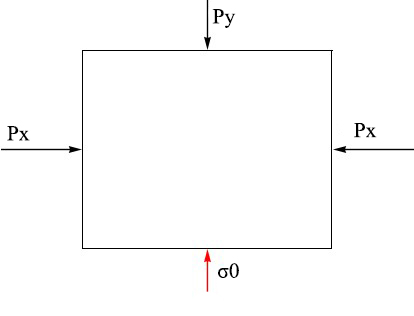
\includegraphics[width=0.5\linewidth]{figures/def4}
\end{center}
	Ciò significa che per mantenere l'equilibrio in direzione $y$, $\sigma_0$ è uno sforzo che agisce nel verso opposto a $P_y$
	\[P_y = -{2\over\sqrt{3}}\sigma_0\]
	E quindi 
	\begin{equation}\label{eq:labstamp}
		\boxed{-P_x+P_y = -{2\over\sqrt{3}}\sigma_0}
	\end{equation}
	Differenziando si ottiene 
	\[ dP_x = dP_y\]
	Che sostituita nell'equazione differenziale (\ref{eq:5}) porta a 
	\[\dfrac{dP_y}{dx} = -2{\tau\over h}\]
	Se l'attrito è esprimibile mediante la teoria Coulombiana, questo si può scrivere come 
	\[\mu = {\tau\over\sigma} = \dfrac{\tau}{P_y}\Rightarrow\tau = \mu P_y\]
	E quindi
	\[\dfrac{dP_y}{dx} = -2{\mu P_y\over h}\]
	Separando le variabili 
	\[\dfrac{dP_y}{P_y} = -2\dfrac{\mu}{h}dx\]
	Integrando tra $x$ ed $L/2$ si ottiene 
	\[P_y = - P_y\left(L\over2\right)\cdot e^{{2\mu\over h}\left({L\over2}-x\right)}\]
	Sapendo che $P_y\left(L\over2\right) = -{2\over\sqrt{3}}\sigma_0$ si arriva a 
	\begin{equation}\label{eq:2}
		P_y = {2\over\sqrt{3}}\sigma_0 \cdot e^{{2\mu\over h}\left({L\over2}-x\right)}
	\end{equation}
	E sostituendo
	\[P_x = {2\over\sqrt{3}}\sigma_0 \cdot \left[e^{{2\mu\over h}\left({L\over2}-x\right)}-1\right]\]
\begin{center}
	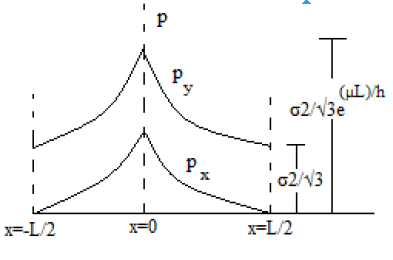
\includegraphics[width=0.5\linewidth]{figures/def5}
\end{center}
	Per $x=0$ l'andamento delle pressioni genera un massimo: quella è la superficie neutra, il materiale in quel punto non si muove e la pressione è la più grande. 

	Notare poi come questa decresca fino a valori minimi: le pressioni non variano durante la lavorazione. 
\newpage	
	\subsection{Laminazione}
	A fronte della riduzione di altezza il materiale scorre nella direzione di laminazione. 
	
	Affinché avvenga laminazione devono esserci forze d'attrito. 
	
	Nell'ipotesi che la laminazione non deformi il materiale lungo l'asse dei rulli, si può applicare lo Slab Method, lo stato è quello di deformazione piana. 
\begin{center}
	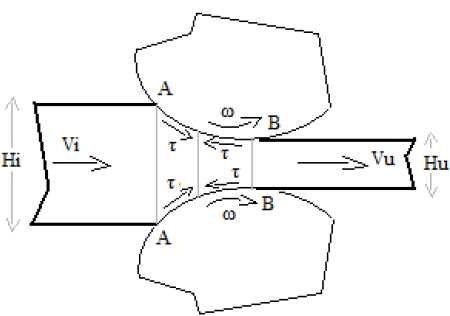
\includegraphics[width=0.5\linewidth]{figures/def6}
\end{center}
	In deformazione plastica si può applicare la conservazione del volume
	\[v_ib_ih_i = v_ub_uh_u\]
	Come detto si pone in direzione assiale ai rulli $b_i=b_u = b$ e allora 
	\[v_ih_i = v_uh_u\]
	Sapendo che $h_i>h_u$ allora varrà 
	\[v_i<v_u\]
	Osservando le velocità lungo l'arco di contatto con il rullo:
	\begin{itemize}\compresslist
		\item Nella sezione di ingresso la velocità dei rulli è maggiore di quella del laminato: le forze tendono a trascinare il materiale tra i rulli
		\item Nella zona centrale la velocità dei rulli e quella della lamiera coincidono
		\item Nella zona finale la velocità dei rulli è inferiore a quella del laminato, il materiale
		tende ad essere rallentato dalle forze d'attrito
	\end{itemize}
\begin{center}
	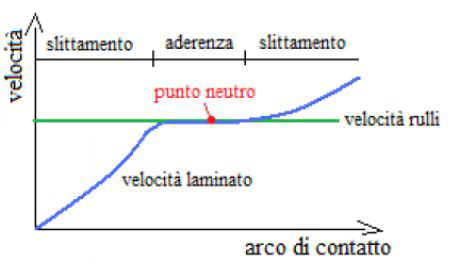
\includegraphics[width=0.5\linewidth]{figures/def7}
\end{center}
	Ciò implica l'esistenza di una sezione, la \textbf{sezione neutra} in corrispondenza alla quale la velocità relativa laminato-cilindri è nulla e le tensioni tangenziali di attrito invertono il loro verso.
\begin{center}
	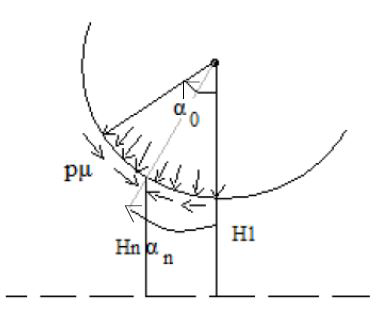
\includegraphics[width=0.5\linewidth]{figures/def8}
\end{center}
	La sezione neutra $S_n$ è una sezione di equilibrio, quindi in direzione orizzontale: 
	\[\int_{\alpha_n}^{\alpha_0}P\mu\cdot\cos\alpha\cdot Rd\alpha - \int_{0}^{\alpha_n}P\mu\cdot\cos\alpha\cdot Rd\alpha - \int_{0}^{\alpha_0}P\cdot\sin\alpha\cdot Rd\alpha = 0\]
	Se $R, P, \mu = cost$ 
	\[\mu\cdot\sin\alpha_0-\sin\alpha_n - \mu\cdot\sin\alpha_n + \cdot\cos\alpha_0-1 = 0\]
	\[\sin\alpha_n = \dfrac{sin\alpha_0}{2} + \dfrac{\cos\alpha_0-1}{2\mu}\]
	Attraverso le formule di bisezione e l'approssimazione in piccoli angoli si ottiene 
	\begin{equation}\label{eq:3}
		\boxed{\alpha_n = {\alpha_0\over2} - {1\over\mu}\left(\alpha_0\over2\right)^2}
	\end{equation}
	Per lavorazioni a caldo si può in buona approssimazione considerare $\mu\rightarrow\infty$ e allora
	\begin{equation}\label{eq:4}
		\boxed{\alpha_n = {\alpha_0\over2}}
	\end{equation}
	\begin{itemize}\compresslist
		\item Se il $\mu\downarrow \Rightarrow S_n\rightarrow S_{\text{out}}$, lungo tutto l'arco di contatto la velocità del rullo è sempre maggiore di quella del laminato, la laminazione avviene ma sarebbe necessario utilizzare delle macchine molto potenti economicamente svantaggiose
		\item Se $\mu\uparrow \Rightarrow S_n\rightarrow S_{\text{in}}$, lungo tutto l'arco di contatto la velocità del laminato è maggiore della velocità periferica del rullo e tutte le azioni tangenziali dovute all'attrito si oppongono al trascinamento e il laminato non imbocca
	\end{itemize}
	È proprio grazie a queste condizioni d'attrito che è possibile stabilire una condizione limite di imbocco per la quale il trascinamento del laminato avverrà automaticamente: la \textbf{condizione di imbocco spontaneo}.
	
	Tale condizione può essere espressa, o secondo il modello coulombiano d'attrito, o attraverso la riduzione dello spessore ottenuto. 
	\newpage
	\subsubsection{Metodo dinamico}\mbox{} \\
\begin{center}
	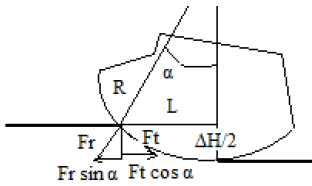
\includegraphics[width=0.3\linewidth]{figures/def9.0}
	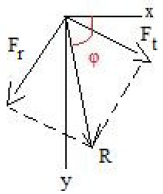
\includegraphics[width=0.2\linewidth]{figures/def9}
\end{center}	
	Da Coulomb
	\[\mu = {\tau\over\sigma} = {F_t\over F_n} = {F_t\over F_r}\]
	Affinché ci sia imbocco spontaneo la componente tangenziale dev'essere maggiore di quella radiale
	\[F_t\cos\alpha>F_r\sin\alpha\]
	\[{F_t\over F_r}>{\sin\alpha\over\cos\alpha} = \tan\alpha\]
	In sostanza 
	\[\mu>\tan\alpha\]
	Potendo definire $\mu$ attraverso il cono d'attrito $\varphi$
	\[\mu = \tan\varphi\]
	Allora
	\[\tan\varphi>\tan\alpha\]
	E la condizione di imbocco spontaneo si traduce in 
	\begin{equation}\label{eq:imb1}
		\boxed{\varphi>\alpha}
	\end{equation}
\newpage
	\subsubsection{Metodo geometrico}\mbox{} \\
\begin{center}
	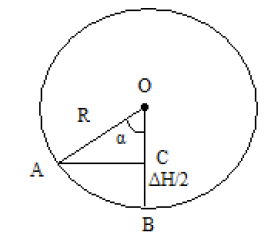
\includegraphics[width=0.5\linewidth]{figures/def10}
\end{center}
	Si può calcolare l'arco di contatto $AB$ come 
	\[\begin{aligned}
		AB^2 = AC^2 + CB^2 &= OA^2 - OC^2 + CB^2\\
		&= R^2 - \left(R-{\Delta H\over2}\right)^2 + \left(\Delta H\ over2\right)^2 \\
		&= R^2 - \left(R^2+{\Delta H^2\over4} - R\Delta H\right) + {\Delta H^2\over4} \\
		& = R\Delta H
	\end{aligned}\]
	Per cui
	\[L = AB = \sqrt{R\Delta H}\]
	Per piccoli angoli è sempre valido $\tan\alpha\approx\alpha$, allora  
	\[\tan\alpha = \alpha = {L\over R} = \sqrt{R\Delta H\over R^2} = \sqrt{\Delta H\over R}\]
	\[\alpha = \sqrt{\Delta H\over R}\]
	Infine, poiché con (\ref{eq:imb1}) si era visto che deve essere $\alpha<\varphi$, si può scrivere una seconda condizione di imbocco spontaneo
	\[\sqrt{\Delta H\over R}<\mu\]
	\begin{equation}\label{eq:imb2}
		\boxed{\Delta H <\mu^2R}
	\end{equation}
	Attraverso lo stesso metodo geometrico è possibile calcolare anche l'altezza della sezione media
	\[\Delta H = 2\cdot{\Delta H\over2} = CB = OB - OC = R - R\cos\alpha = R(1-\cos\alpha)\] 
	\[\Delta H = H_n - H_f \Rightarrow H_n = H_f + \Delta H = H_f + R(1-\cos\alpha)\]
	E la sezione neutra diviene pari a 
	\[S_n = H_nb\]
	\newpage
	\subsection{Estrusione}
	Nell'estrusione si applica uno sforzo di compressione a monte della matrice
\begin{center}
	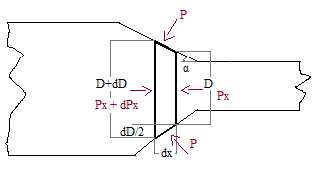
\includegraphics[width=0.8\linewidth]{figures/def11}
\end{center}
	L'equilibrio delle forze lungo la direzione di estrusione, considerando la matrice tronco-sferica è pari a
	\[(P_x+dP_x)\pi\dfrac{(D+dD)^2}{4} - P_x\pi{D^2\over4} - P\pi D\dfrac{dD}{2\sin\alpha}\sin\alpha-P\mu\pi D\dfrac{dD}{2\sin\alpha}\cos\alpha=0\]
	Semplificando e trascurando gli infinitesimi di ordine superiore si ottiene:
	\[dP_x{D\over4} + P_x{dD\over2}-{P\over2}dD - P\mu\cot\alpha{dD\over2} = 0\]
	\begin{equation}\label{eq:7}
		dP_xD + 2[P_x-P(1+\mu\cot\alpha)]dD=0
	\end{equation}
	Per poter calcolare le pressioni, dato che lo stato tensionale è tridimensionale e non è possibile applicare lo Slab Method, si ipotizza la matrice sferica e si applica l'ipotesi di Sachs per cui lo stato deformativo è sferico:
	\[P = P_r = P_\theta\]
	Ipotizzano che le direzioni di applicazione dei carichi siano direzioni principali:
	\[\sigma_1 = P\qquad\sigma_2 = P_r\qquad\sigma_3=P_\theta \Rightarrow \sigma_2=\sigma_3\]
	Ricordando che per Von Mises si ha deformazione plastica quando 
	\[(\sigma_1-\sigma_2)^2+(\sigma_2-\sigma_3)^2+(\sigma_3-\sigma_1)^2 = 2\sigma^2_0\]
	Per cui
	\[(\sigma_1-\sigma_2)^2+(\sigma_3-\sigma_1)^2 = 2\sigma^2_0\]
	\[2(\sigma_1-\sigma_2)^2 = 2\sigma^2_0\]
\begin{equation}\label{eq:6}
	\boxed{	\sigma_1-\sigma_2 = \pm\sigma_0}
\end{equation}
	Poiché gli sforzi subiti dal parallelepipedo infinitesimo sono entrambi di compressione è possibile scrivere
\begin{center}
	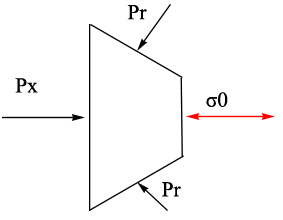
\includegraphics[width=0.5\linewidth]{figures/def11.1}
\end{center}	
	\[\sigma_1 = -P_x\qquad\sigma_2 = -P_r\]
	E allora l'equazione di Von Mises diviene
	\[-P_x-(-P_r) = \pm\sigma_0\]
	\[-P_x+P_r = \pm\sigma_0\]
	Ad $x = OUT, ~P_x=0$ all'uscita della matrice il corpo non subisce più alcuna pressione
	\[P_r = \pm\sigma_0\]
\begin{center}
	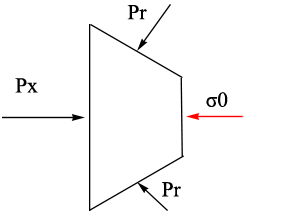
\includegraphics[width=0.5\linewidth]{figures/def11.2}
\end{center}
	Ciò significa che per far avvenire la deformazione plastica, $\sigma_0$ è uno sforzo che agisce concorde alla risultante delle due $P_r$
	\[P_r = +\sigma_0\]
	E quindi 
	\[-P_x+P_r = +\sigma_0\]
	Ovvero
	\begin{equation}\label{eq:slabest}
		\boxed{P_x-P_r = -\sigma_0}
	\end{equation}
	È possibile ricavare adesso la pressione da (\ref{eq:7}), perché dalle ipotesi di Sachs $P = P_r$
	\[{dD\over D} = \dfrac{dP_x}{2[P_x-P_r(1+\mu\cot\alpha)]}\]
	\[{dD\over D} = \dfrac{dP_x}{2[P_x-(P_r+P_x-P_x)(1+\mu\cot\alpha)]}\]
	\[{dD\over D} = \dfrac{dP_x}{2[P_x-P_x(1+\mu\cot\alpha)-(P_r+P_x)(1+\mu\cot\alpha)]}\]
	\[{dD\over D} = \dfrac{dP_x}{2[P_x-P_x(1+\mu\cot\alpha)-\sigma_0(1+\mu\cot\alpha)]}\]
	Facendo opportune considerazioni sui segni degli sforzi
	\[{dD\over D} = \dfrac{dP_x}{2P_x\mu\cot\alpha+2\sigma_0(1+\mu\cot\alpha)]}\]
	Integrando
	\[\int_{D_i}^{D_f}{dD\over D} = \int_{P_{x0}}^{0}\dfrac{dP_x}{2P_x\mu\cot\alpha+2\sigma_0(1+\mu\cot\alpha)]}\]
	\begin{equation}\label{eq:9}
		\boxed{P_{x0} = \sigma_0\dfrac{1+\mu\cot\alpha}{\mu\cot\alpha}\left[\left(D_i\over D_f\right)^{2\mu\cot\alpha}-1\right]}
	\end{equation}
	Ottenendo come risultato la pressione assiale che deve fornire lo spintore per far avvenire la deformazione.
	
	\newpage
	
	\subsection{Trafilatura}
	Nella trafilatura si applica uno sforzo di trazione a valle della matrice.
\begin{center}
	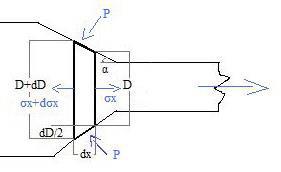
\includegraphics[width=0.5\linewidth]{figures/def12}
\end{center}
	L'equilibrio delle forze lungo la direzione di estrusione, considerando la matrice tronco-sferica è pari a
	\[(P_x+dP_x)\pi\dfrac{(D+dD)^2}{4} - P_x\pi{D^2\over4} - P\pi D\dfrac{dD}{2\sin\alpha}\sin\alpha-P\mu\pi D\dfrac{dD}{2\sin\alpha}\cos\alpha=0\]
	Semplificando e trascurando gli infinitesimi di ordine superiore si ottiene:
	\[dP_x{D\over4} + P_x{dD\over2}-{P\over2}dD - P\mu\cot\alpha{dD\over2} = 0\]
	\begin{equation}\label{eq:8}
		dP_xD + 2[P_x-P(1+\mu\cot\alpha)]dD=0
	\end{equation}
	Per poter calcolare le pressioni, dato che lo stato tensionale è tridimensionale e non è possibile applicare lo Slab Method, si ipotizza la matrice sferica e si applica l'ipotesi di Sachs per cui lo stato deformativo è sferico:
	\[P = P_r = P_\theta\]
	La condizione di plasticità di Von Mises si traduce sempre in (\ref{eq:6})
	\[\sigma_1-\sigma_2 = \pm\sigma_0\]
	Ora gli sforzi subiti dal parallelepipedo infinitesimo sono di trazione e di compressione, allora è possibile scrivere
	\begin{center}
		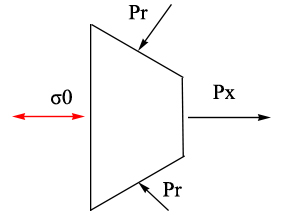
\includegraphics[width=0.5\linewidth]{figures/def12.1}
	\end{center}
	\[\sigma_1 = P_x\qquad\sigma_2 = -P_r\]
	E allora l'equazione di Von Mises diviene
	\[P_x-(-P_r) = \pm\sigma_0\]
	\[P_x+P_r = \pm\sigma_0\]
	Ad $x = IN, ~ P_x=0$ all'entrata della matrice il corpo non subisce alcuna pressione
	\[P_r = \pm\sigma_0\]
	\begin{center}
		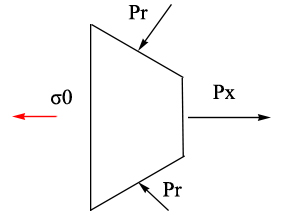
\includegraphics[width=0.5\linewidth]{figures/def12.2}
	\end{center}
	Ciò significa che per far avvenire la deformazione plastica, $\sigma_0$ è uno sforzo che agisce concorde alla risultante delle due $P_r$
	\[P_r = +\sigma_0\]
	E quindi 
	\begin{equation}\label{eq:slatr}
		\boxed{P_x+P_r = +\sigma_0}
	\end{equation}
	Per conoscere la pressione assiale che deve fornire la bobina avvolgicavo per far avvenire la trafilatura, basta muoversi similmente a quanto fatto per l'estrusione e si ottiene
	\begin{equation}\label{eq:10}
		\boxed{P_{x0} = \sigma_0\dfrac{1+\mu\cot\alpha}{\mu\cot\alpha}\left[1-\left(D_f\over D_i\right)^{2\mu\cot\alpha}-1\right]}
	\end{equation}
	\newpage
	\part{Asportazione di materiale}
	Il taglio dei metalli ha lo scopo di mutare forma e dimensioni di un materiale attraverso l'utilizzo di un utensile con tagliente. \\
	
	Analizzando i meccanismi del taglio ortogonale libero, si possono individuare, tra cuneo e pezzo, un petto e un dorso.
	
	Tra questi si possono identificare gli angoli $\alpha, \gamma, \phi, \beta$
\begin{center}
	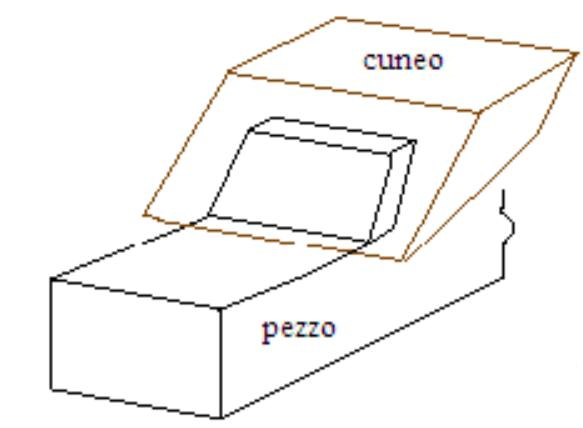
\includegraphics[width=0.4\linewidth]{figures/asp1}
	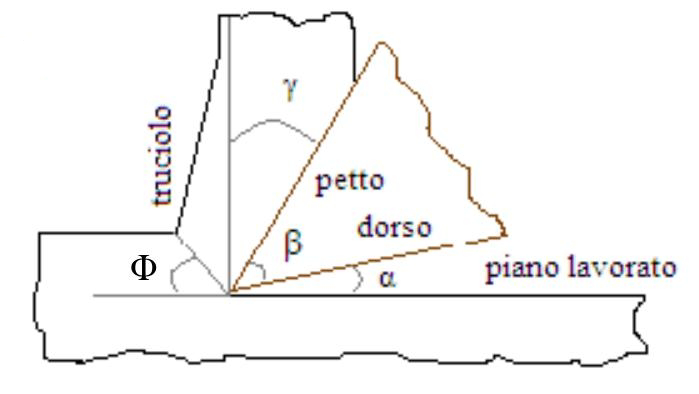
\includegraphics[width=0.4\linewidth]{figures/asp2}
\end{center}
\begin{itemize}\compresslist
	\item $\gamma$ \textbf{angolo di spoglia superiore}: compreso tra la verticale e il petto dell'utensile, determina le forze di taglio in gioco
	
	\item $\phi$ \textbf{angolo di scorrimento}: rappresenta il piano dove scorrono le dislocazioni
	
	\item $\alpha$ \textbf{angolo di spoglia inferiore principale}: compreso tra la superficie lavorata e il dorso dell'utensile.
	
	Se $\alpha=0$ il dorso entra in contatto con la superficie lavorata. 
	
	\item $\beta$ \textbf{angolo di tagliente}: fornisce informazioni sulla robustezza del tagliente
	\[\beta = 90\degree - (\alpha+\gamma)\]
\end{itemize}
	Va da se che per materiali duttili $\gamma\uparrow\beta\downarrow$ e il tagliente sarà più affilato, invece per materiali fragili $\gamma\downarrow\beta\uparrow$ servono sezioni dell'utensile maggiori per evitarne il danneggiamento.\\
	
	Per studiare il taglio si impongono le seguenti ipotesi semplificative:
	\begin{itemize}\compresslist
		\item Tagliente perfettamente affilato
		\item Velocità di taglio costante
		\item Profondità di passata costante
		\item volume di materiale costante
		\item Materiale isotropo
		\item Effetti di bordo trascurabili: la larghezza del cuneo è superiore a quella del materiale
		\item Deformazione piana: la larghezza del truciolo rimane uguale alla larghezza iniziale del pezzo
	\end{itemize}
\newpage
	La tipologia di truciolo fornisce informazioni sul tipo di materiale lavorato:
\begin{center}
	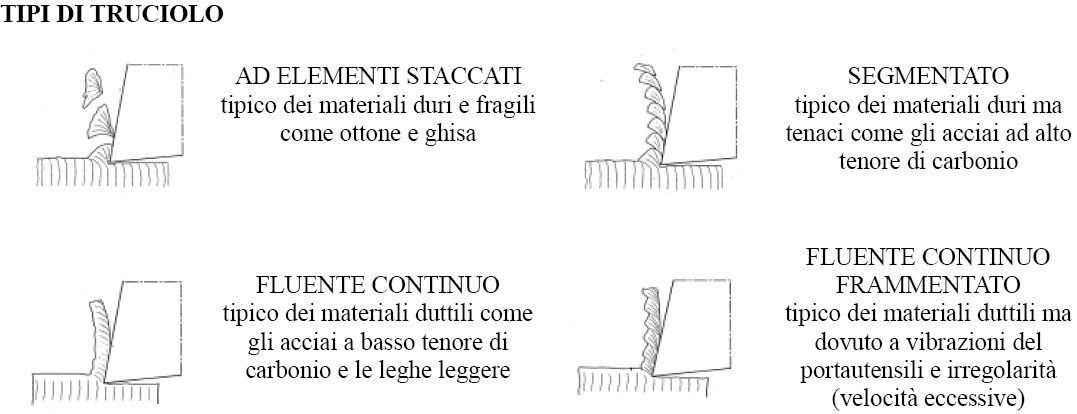
\includegraphics[width=1.2\linewidth]{figures/asp3}
\end{center}

\section{Angolo di scorrimento}
	La deformazione plastica del materiale avviene per scorrimento e l'angolo di scorrimento $\phi$ individua il piano di scorrimento; questo è calcolabile conoscendo altezza di passata $s$ e l'altezza del truciolo $s_1$. 
	
	Si definisce il fattore di ricalcamento $c$:
	\begin{equation}\label{eq:11}
		c = {s\over s_1}
	\end{equation}
	Imponendo la conservazione del volume 
	\[sbL=s_1b_1L_1\]
	Poiché ci si è posti nel caso di deformazione piana, la larghezza del truciolo rimane invariata $b=b_1$ e allora 
	\[c = {s\over s_1} = {L\over L_1}\]
	\newpage
\begin{center}
	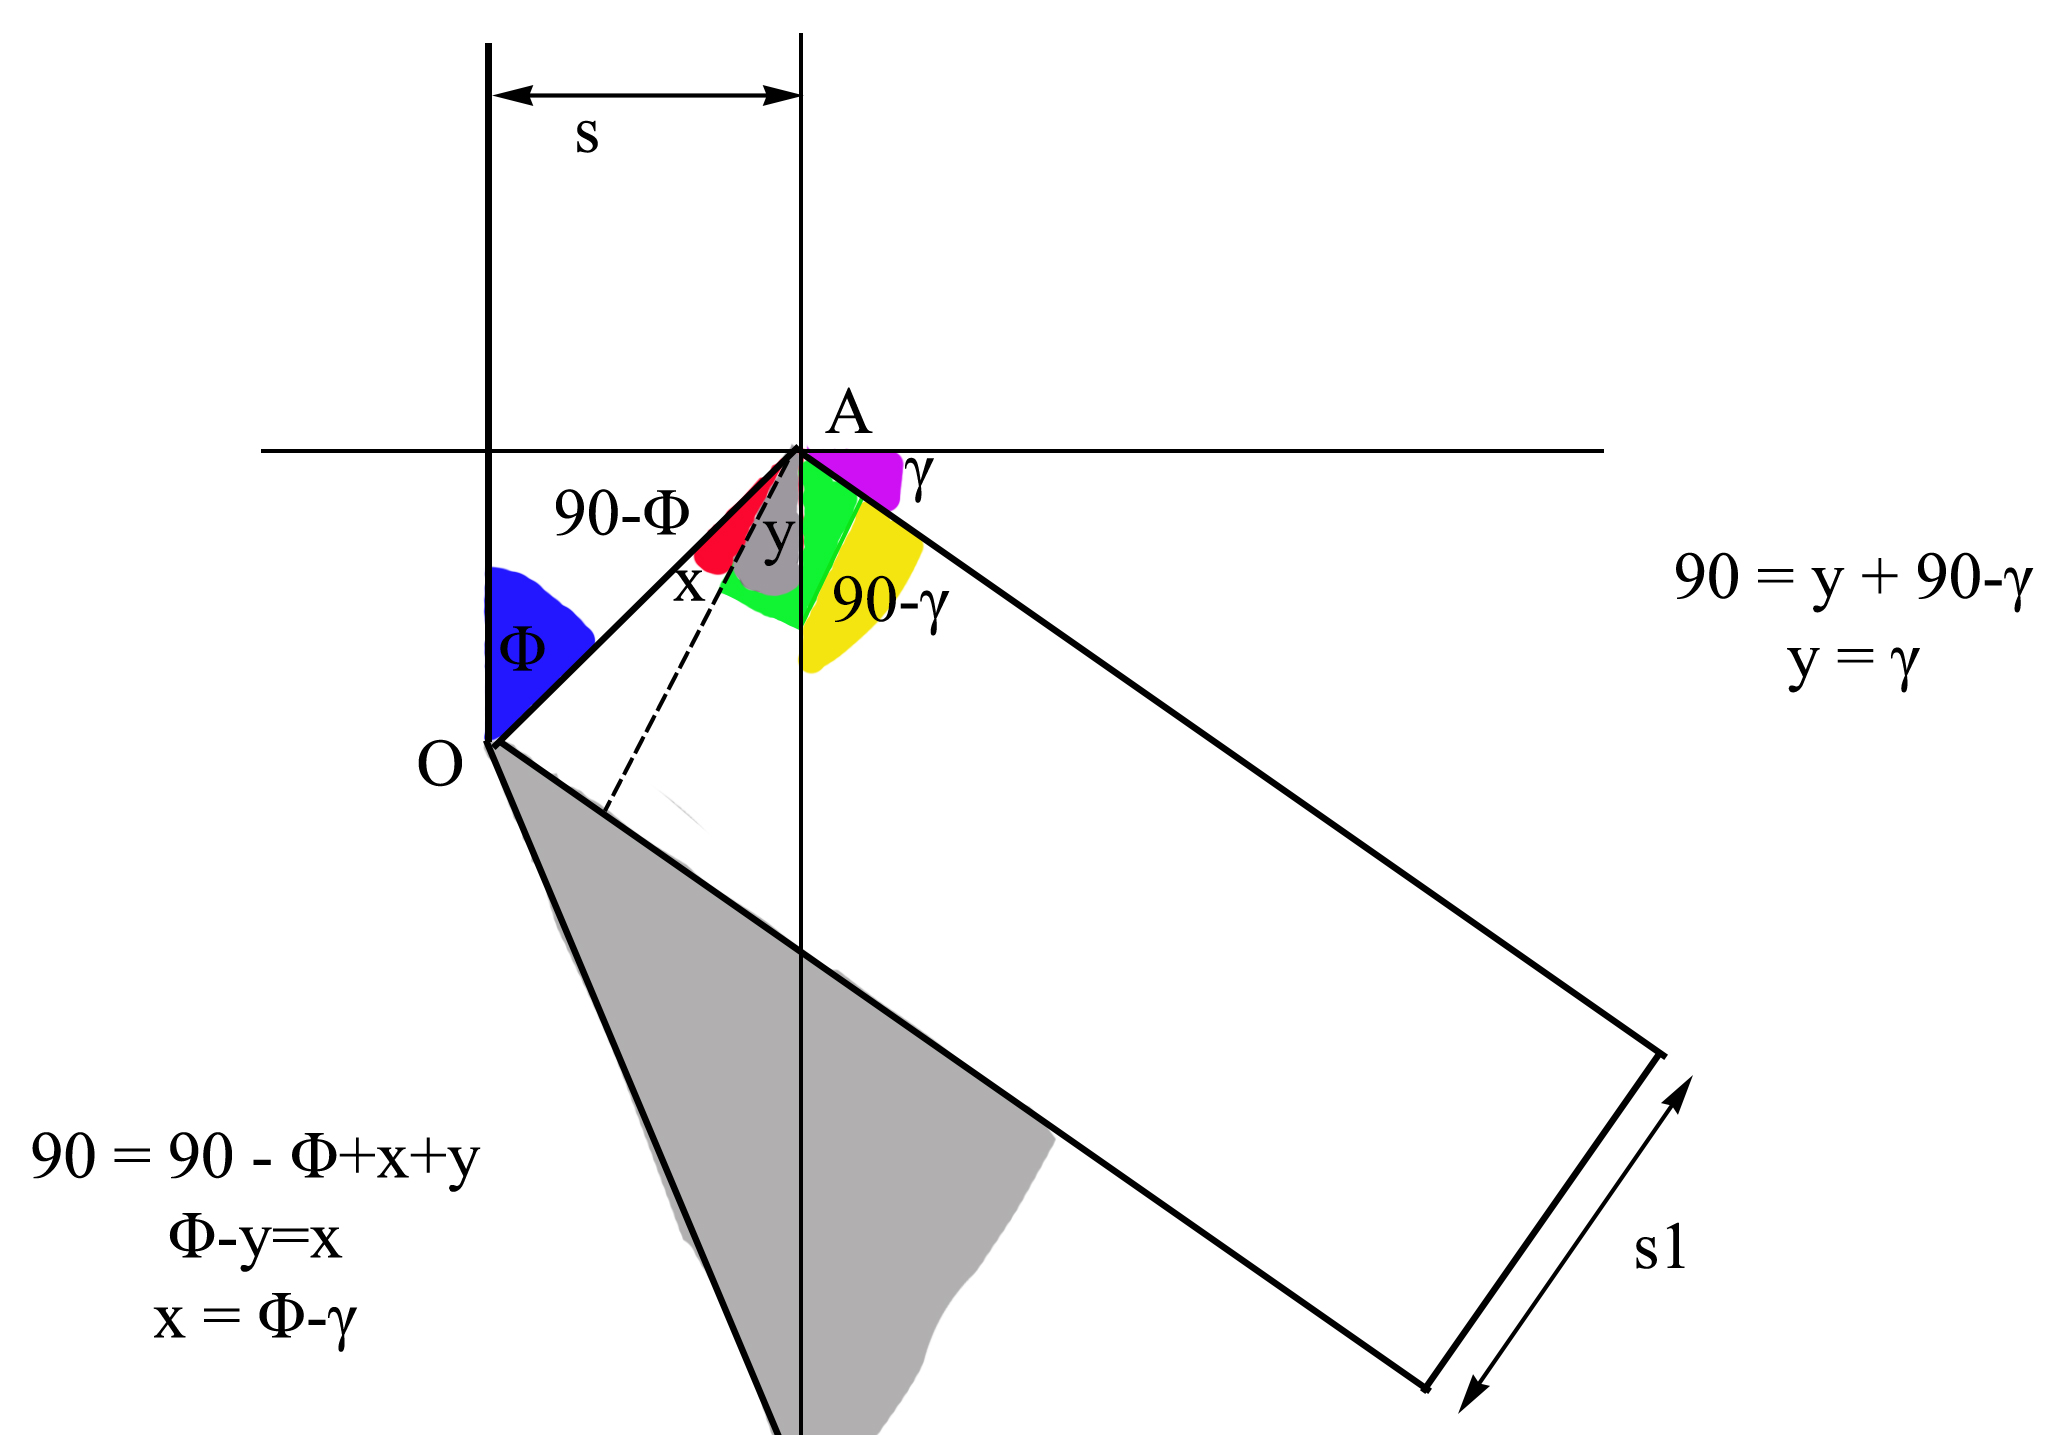
\includegraphics[width=0.55\linewidth]{figures/asp4.0}
	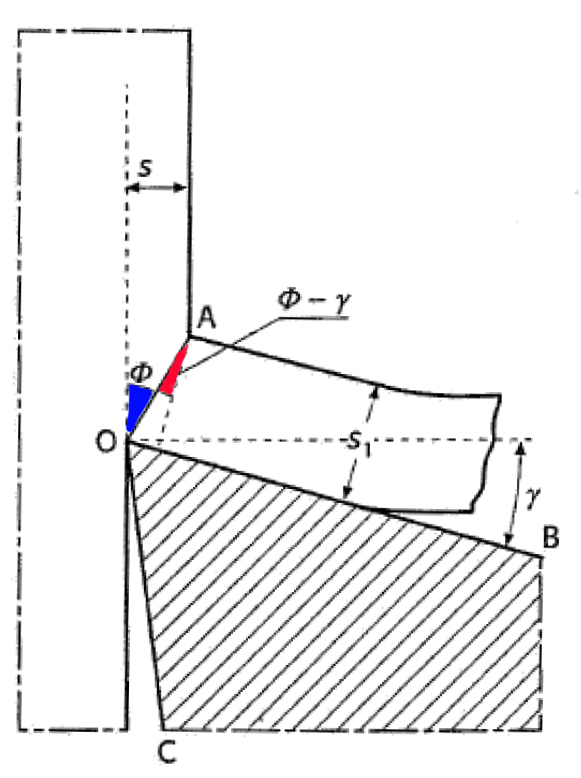
\includegraphics[width=0.4\linewidth]{figures/asp4}
\end{center}
	È possibile correlare il fattore di ricalcamento $c$ all'angolo $\phi$ esprimendo gli spessori $s$ ed $s_1$ attraverso delle relazioni trigonometriche in funzione dell'ipotenusa $OA$
	\[c = {s\over s_1} = \dfrac{OA\sin\phi}{OA\cos(\phi-\gamma)}\]
	Dalle formule della sottrazione
	\[\cos(\phi-\gamma) = \cos\phi\cos\gamma + \sin\phi\sin\gamma\] 
	Per cui
	\[c = \dfrac{\sin\phi}{\cos\phi\cos\gamma + \sin\phi\sin\gamma}\]
	\[c(\cos\phi\cos\gamma + \sin\phi\sin\gamma) = \sin\phi\]
	\[c\cos\phi\left(\cos\gamma + \dfrac{\sin\phi\sin\gamma}{\cos\phi}\right) = \sin\phi \]
	\[c(\cos\gamma + \tan\phi\sin\gamma) = \dfrac{\sin\phi}{\cos\phi} \]
	\[c(\cos\gamma + \tan\phi\sin\gamma) = \tan\phi \]
	\[\tan\phi - c\tan\phi\sin\gamma = c\cos\gamma\]
	\[\tan\phi(1-c\sin\gamma) = c\cos\gamma\]
	\begin{equation}\label{eq:12}
		\boxed{\tan\phi = \dfrac{c\cos\gamma}{1-c\sin\gamma}}
	\end{equation}
	Noto quindi il fattore di ricalcamento $c$ e l'angolo di spoglia superiore $\gamma$ è possibile risalire all'angolo di scorrimenti $\phi$.
	\newpage
	\section{Modello di Pijspanen}
	Si immagina il materiale come composto da tante lamelle di spessore finito, l'avanzamento dell'utensile sospinge ciascun elemento in avanti, obbligandolo a scorrere sull'elemento successivo
\begin{center}
	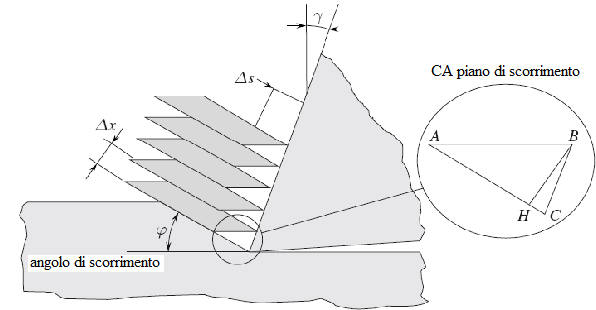
\includegraphics[width=0.5\linewidth]{figures/asp5}
\end{center}
	La forza che l'utensile applica sul truciolo dev'essere  in grado di generare sul piano $CA$, una tensione tangenziale necessaria e sufficiente a provocare lo scorrimento relativo tra le lamelle del materiale.\\
	
	Il modello di Pijspanen si basa sull'esistenza di un unico piano di
	scorrimento, ipotesi in prima approssimazione avvalorata dato che l'estensione della zona di scorrimento tende a un unico piano per i valori delle
	velocità di taglio comunemente impiegati.\\
	
	La deformazione plastica può essere vista come il rapporto tra lo spostamento orizzontale $\Delta s$ e quello verticale $\Delta x$
	\[\gamma_s = \dfrac{\Delta s}{\Delta x}\] 
	In questa trattazione $\Delta s$ è la distanza sul piano di scorrimento, mentre $\Delta x$ è la distanza verticale tra le lamelle.
\begin{center}
	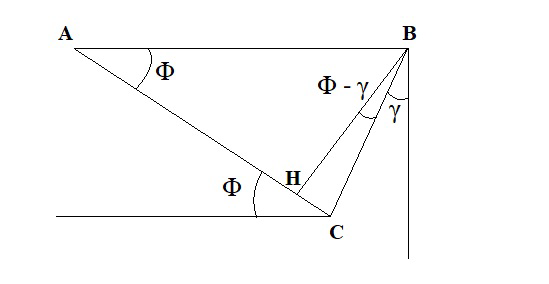
\includegraphics[width=0.5\linewidth]{figures/asp6}
\end{center}
	\[\begin{matrix}
		\Delta s = AH + HC & \qquad & \Delta x = BH\\
		AH = AB\cos\phi & \qquad & BH = AB\sin\phi \\
		HC = BH\tan(\phi-\gamma) & & \\
	\end{matrix}\]
	Per cui
	\[\begin{aligned}
		\gamma_s  = \dfrac{AB\cos\phi+BH\tan(\phi-\gamma)}{BH} &= \dfrac{AB\cos\phi}{BH} + \dfrac{BH\tan(\phi-\gamma)}{BH} = \\
		& = \dfrac{AB\cos\phi}{AB\sin\phi} + \tan(\phi-\gamma) \\
		& = \cot\phi + \tan(\phi-\gamma)
	\end{aligned} 
	\] 
	\begin{equation}\label{eq:13}
		\gamma_s = \cot\phi + \tan(\phi-\gamma)
	\end{equation}
	Lo studio della derivata di questa quantità fornisce l'angolo di scorrimento tale da minimizzare lo scorrimento stesso e quindi l'entità della deformazione plastica e conseguentemente il lavoro di deformazione. 
	\[\dfrac{d\gamma_s}{dt} = 0 \Leftrightarrow -\dfrac{1}{\sin^2\phi} + \dfrac{1}{\cos^2(\phi-\gamma)} = 0\]
	\[\sin^2\phi - \cos^2(\phi-\gamma) = 0\]
	\[\left[\sin\phi-\cos(\phi-\gamma)\right]\left[\sin\phi+\cos(\phi-\gamma)\right] = 0\]
	Si prende in considerazione l'equazione che ha soluzione nel primo quadrante:
	\[\sin\phi-\cos(\phi-\gamma)=0\]
	Ricordando che \(\cos\theta = \sin({\pi\over2}-\theta)\) si può scrivere
	\[\sin\phi-\sin({\pi\over2}-\phi+\gamma)=0\]
	\[\phi = {\pi\over2}-\phi+\gamma\]
	Ovvero, la relazione di Pijspanen 
	\begin{equation}\label{eq:14}
		\boxed{2\phi-\gamma = {\pi\over2}}
	\end{equation}
	Inoltre, ponendo $\gamma=0$ si ottiene 
	\[\phi= {\pi\over4}=45\degree\]
	Ma da (\ref{eq:12})
	\[\tan\phi = \dfrac{c\cos\gamma}{1-c\sin\gamma} \Rightarrow c=1 \Rightarrow s=s_1\]
	Ed il lavoro di deformazione plastica è il minimo. 
	\newpage
\begin{center}
	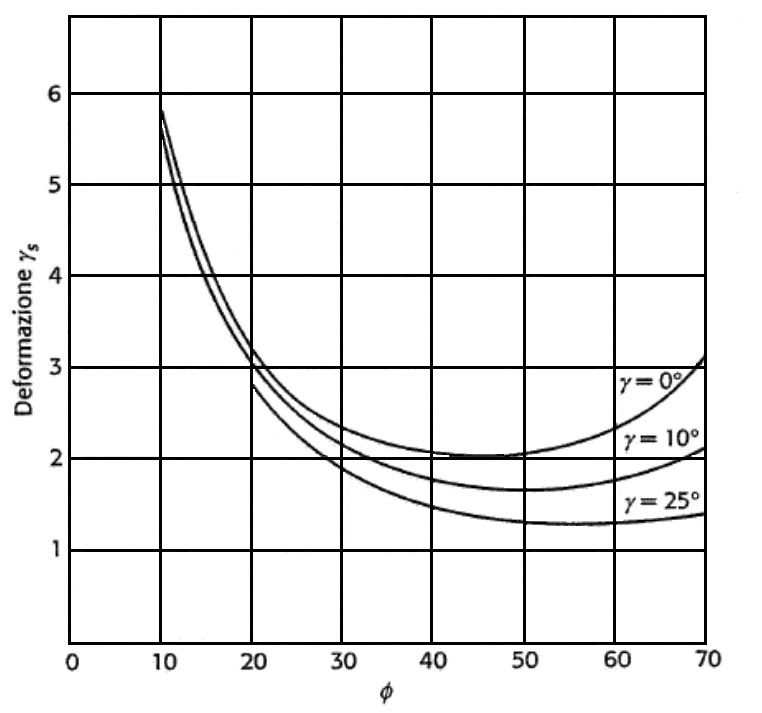
\includegraphics[width=0.5\linewidth]{figures/asp7}
\end{center}
	\begin{itemize}\compresslist
		\item \(\phi\downarrow ~ \gamma_s\uparrow\) aumenta l'energia dispersa per effettuare deformazione plastica
		\item \(\phi\uparrow ~ \gamma_s\downarrow\) diminuisce l'energia dispersa per effettuare deformazione plastica
	\end{itemize}
	\begin{itemize}\compresslist
		\item $\gamma \uparrow$ significa avere un utensile più affilato
		\item $\phi\uparrow$ significa che la dimensione del piano lungo il quale sta avvenendo lo scorrimento diminuisce, significa avere una diminuzione del segmento $OA$ e quindi che si devono spostare meno atomi con forze minori da applicare
	\end{itemize}
	\newpage
	\section{Modello di Merchant}
	Se si considera il truciolo come un corpo libero, questo, istante per istante, dovrà
	essere in equilibrio sotto l'azione delle forze applicate dall'utensile e quelle di resistenza sviluppate dal materiale.
\begin{center}
	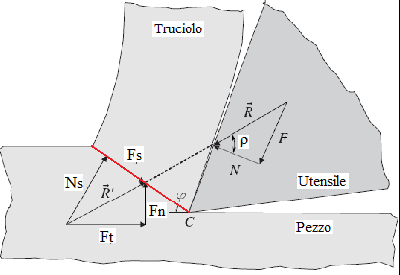
\includegraphics[width=0.5\linewidth]{figures/asp8}
\end{center}
	In cui si identificano delle forze di attrito:
	\begin{itemize}\compresslist
 	\item $F$ Forza tangenziale, parallela al petto dell'utensile 
 	\item $N$ Forza normale, perpendicolare al petto dell'utensile 
 	\item $\rho$ Cono d'attrito
 	\end{itemize}
 	Delle forze relative al piano di scorrimento:
 	\begin{itemize}\compresslist
 		\item $F_s$ Forza da fornire per far avvenire la deformazione plastica e quindi muovere atomi e dislocazioni lungo il piano di scorrimento, parallela al piano di scorrimento
 		\item $N_s$ Forza normale al piano di scorrimento, influenza il fattore di ricalcamento $c$
 	\end{itemize}
 	Delle forze sul tagliente
 	\begin{itemize}\compresslist
 		\item $F_t$ Forza necessaria all'avanzamento del tagliente 
 		\item $F_n$ Forza che tende a sollevare l'utensile, repulsione o ritorno elastico
 	\end{itemize}
	\begin{center}
		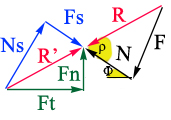
\includegraphics[width=0.5\linewidth]{figures/asp8.1}
	\end{center}
	\begin{en}
		Il modello di Merchant prevede di inscrivere, proiettando, tutte le forze in gioco nell'asportazione di materiale all'interno di una circonferenza tangente al tagliente avente come diametro il modulo della risultante delle forze, questa uguale per tagliente e truciolo.
	\end{en}
\begin{center}
	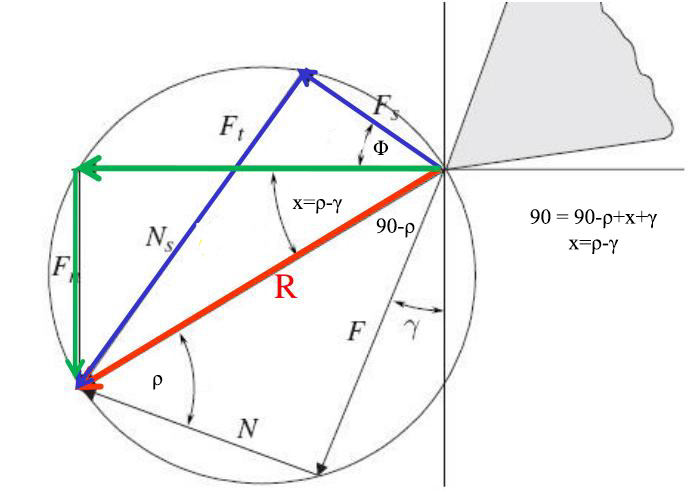
\includegraphics[width=0.5\linewidth]{figures/asp9}
\end{center}
	In questo modo è possibile esprimere il valore di tutte le forze avendo noti gli angoli $\phi, \gamma, \rho$
	\begin{equation}\label{eq:15}
		\begin{cases}
		F_s = R\cos(\phi+\rho-\gamma)\\
		N_s = R\sin(\phi+\rho-\gamma)
	\end{cases}\qquad \begin{cases}
	F_t = R\cos(\rho-\gamma)\\
	F_n = R\sin(\rho-\gamma)
	\end{cases}\qquad\begin{cases}
	F = R\cos(\rho)\\
	N = R\sin(\rho)
	\end{cases}
	\end{equation}
\subsection{I modello di Merchant}
	Si avrà deformazione plastica del truciolo, e quindi taglio, appena sul piano di scorrimento si raggiunge la \textbf{tensione dinamica di scorrimento} $\tau_s$.
	
	A questa tensione è possibile associare la forza $F_s$
	\[F_s = \tau_sA_s = \tau_s\dfrac{A_0}{\sin\phi}\]
	In cui $A_s \approx OA$ è la sezione di materiale deformata plasticamente lungo il piano di scorrimento e $A_0$ è l'area della sezione del truciolo prima del taglio. 
	
	Quindi
	\[R\cos(\phi-\rho-\gamma) = \tau_s\dfrac{A_0}{\sin\phi}\]
	E allora 
	\begin{equation}\label{eq:16}
		R = \dfrac{\tau_sA_0}{\sin\phi\cos(\phi+\rho-\gamma)}
	\end{equation}
	Nota la risultante, la si può sostituire in (\ref{eq:15}) e trovare
	\[F_t = \tau_s\dfrac{A_0\cos(\rho-\gamma)}{\sin\phi\cos(\phi+\rho-\gamma)}\qquad F_n = \tau_s\dfrac{A_0\sin(\rho-\gamma)}{\sin\phi\cos(\phi+\rho-\gamma)}\]
	Affinché avvenga la deformazione plastica si ipotizza che il piano di scorrimento si disponga in modo tale da massimizzare il $\tau_s$ su di esso agente, se ne ricava una condizione che deve essere soddisfatta
	\[\dfrac{dF_n}{d\phi} = 0\]
	\[{d\over d\phi}\left[\tau_s\dfrac{A_0\sin(\rho-\gamma)}{\sin\phi\cos(\phi+\rho-\gamma)}\right] \approx {d\over d\phi} \left[\dfrac{1}{\sin\phi\cos(\phi+\rho-\gamma)}\right] = \]
	\[ = \dfrac{\cos\phi\cos(\phi+\rho-\gamma)-\sin\phi\sin(\phi+\rho-\gamma)}{\sin^2\phi\cos^2(\phi+\rho-\gamma)} = 0 \Leftrightarrow \cos\phi\cos(\phi+\rho-\gamma)-\sin\phi\sin(\phi+\rho-\gamma)=0\]
	Ricordando che 
	\[\begin{cases}
		\cos\alpha\cos\beta=\dfrac{\cos(\alpha+\beta)+\cos(\alpha-\beta)}{2}\\
	\sin\alpha\sin\beta=\dfrac{\cos(\alpha-\beta)-\cos(\alpha+\beta)}{2}
	\end{cases} \]	
	Allora
	\[\cos\phi\cos(\phi+\rho-\gamma)=\sin\phi\sin(\phi+\rho-\gamma)\]
	\[\dfrac{\cos(\phi+\phi+\rho-\gamma)}{2} + \cancel{\dfrac{\cos(\phi-\phi-\rho+\gamma)}{2}} = \cancel{\dfrac{\cos(\phi-\phi-\rho+\gamma)}{2}} - \dfrac{\cos(\phi+\phi+\rho-\gamma)}{2}\]
	\[\cos(2\phi+\rho-\gamma) = 0 \]
	\begin{equation}\label{eq:17}
		\boxed{2\phi+\rho-\gamma = {\pi\over2}}
	\end{equation}
	Il modello di Merchant presenta però una discordanza tra i valori teorici ottenuti applicando tale approccio e i valori sperimentali.
\subsection{II modello di Merchant}	
	Questa discordanza è dovuta proprio alla tensione tangenziale $\tau_s$ necessaria a provocare lo scorrimento, che non è una quantità costante ma funzione della
	tensione normale che agisce sul medesimo piano di scorrimento, secondo la relazione
	\[\tau_s = \tau_{s0}+K\sigma_s\]
\begin{center}
	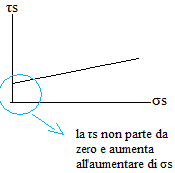
\includegraphics[width=0.3\linewidth]{figures/asp10}
\end{center}
	Merchant nel suo primo modello considera $\tau_s$  come costante, ma nel momento in cui si ha una componente normale al piano di scorrimento, questa avvicina gli atomi tra loro e conseguentemente ciò comporta un aumento della tensione di taglio necessaria allo scorrimento (\ref{eq:1}): le celle elementari vengono compresse e il parametro di cella $a$ diminuisce. \\
	
	La condizione si traduce adesso nell'imporre che il piano di scorrimento si disponga in modo che sia massima la funzione
	\[\tau_{s0} = \tau_s-K\sigma_s\]
	\[{d\over d\phi}\left[\tau_s-K\sigma_s\right] = 0\]
	\begin{equation}\label{eq:19}
		\boxed{2\phi+\rho-\gamma = \arctan\left(1\over K\right)=C}
	\end{equation}
	\begin{center}
		{\small \textit{Dimostrazione non fatta sulle slide, forse interessa solo il risultato? Ma per capire, magari un'occhiata va data...}}
	\end{center}
	Essendo:
	\[\tau_s = {F_s\over A_s} = {R\over A_s}\cos(\phi+\rho-\gamma) = {R\over A_0}\cos(\phi+\rho-\gamma)\sin\phi\approx\cos(\phi+\rho-\gamma)\sin\phi\]
	\[\sigma_s = {N_s\over A_s} = {R\over A_s}\sin(\phi+\rho-\gamma) = {R\over A_0}\sin(\phi+\rho-\gamma)\sin\phi\approx\sin(\phi+\rho-\gamma)\sin\phi\]
	Allora 
	\[{d\over d\phi}\left[\tau_s-K\sigma_s\right] = 0\]
	\[{d\over d\phi}\left[\cos(\phi+\rho-\gamma)\sin\phi-K\sin(\phi+\rho-\gamma)\sin\phi\right]=0\]
	\[
		-\sin(\phi+\rho-\gamma)\sin\phi + \cos(\phi+\rho-\gamma)\cos\phi - K\left[\cos(\phi+\rho-\gamma)\sin\phi + \sin(\phi+\rho-\gamma)\cos\phi\right]=0\]
	\[\begin{split}\cancel{\dfrac{\cos(\phi+\rho-\gamma-\phi)}{2}} + \dfrac{\cos(\phi+\rho-\gamma+\phi)}{2} + \dfrac{\cos(\phi+\rho-\gamma+\phi)}{2} + \cancel{\dfrac{\cos(\phi+\rho-\gamma-\phi)}{2}} - \\ -K\left[\dfrac{\sin(\phi+\rho-\gamma+\phi)}{2} + \cancel{\dfrac{\sin(\phi-\rho+\gamma-\phi)}{2}} + \cancel{\dfrac{\sin(\phi+\rho-\gamma-\phi)}{2}} + \dfrac{\sin(\phi+\rho-\gamma+\phi)}{2} \right] = 0
	\end{split}\]
	\[\cos{2\phi+\rho-\gamma} - K\sin(2\phi+\rho-\gamma) = 0\]
	\[\dfrac{\sin(2\phi+\rho-\gamma)}{\cos{2\phi+\rho-\gamma}} = {1\over K}\]
	\[\tan(2\phi+\rho-\gamma) = {1\over K}\]
	\[2\phi+\rho-\gamma = \arctan\left(1\over K\right)=C\]
	\newpage
	\subsection{Metodo inverso}
	In generale la relazione di Merchant è di difficile applicazione pratica, nonostante ciò in tutta questa trattazione è possibile estrapolare un fatto pratico davvero importante: si può scomporre la risultante anche secondo gli assi individuati dall'utensile, in questo modo si possono misurare attraverso la semplice applicazione di celle di carico $F_t$ ed $F_n$ e da esse calcolare tutte le altre forze in base alle relazioni di Merchant (\ref{eq:15}).
	
	La misura delle forze $F_t$ ed $F_n$ permette inoltre di calcolare l'angolo di
	attrito $\rho$.
	\begin{center}
		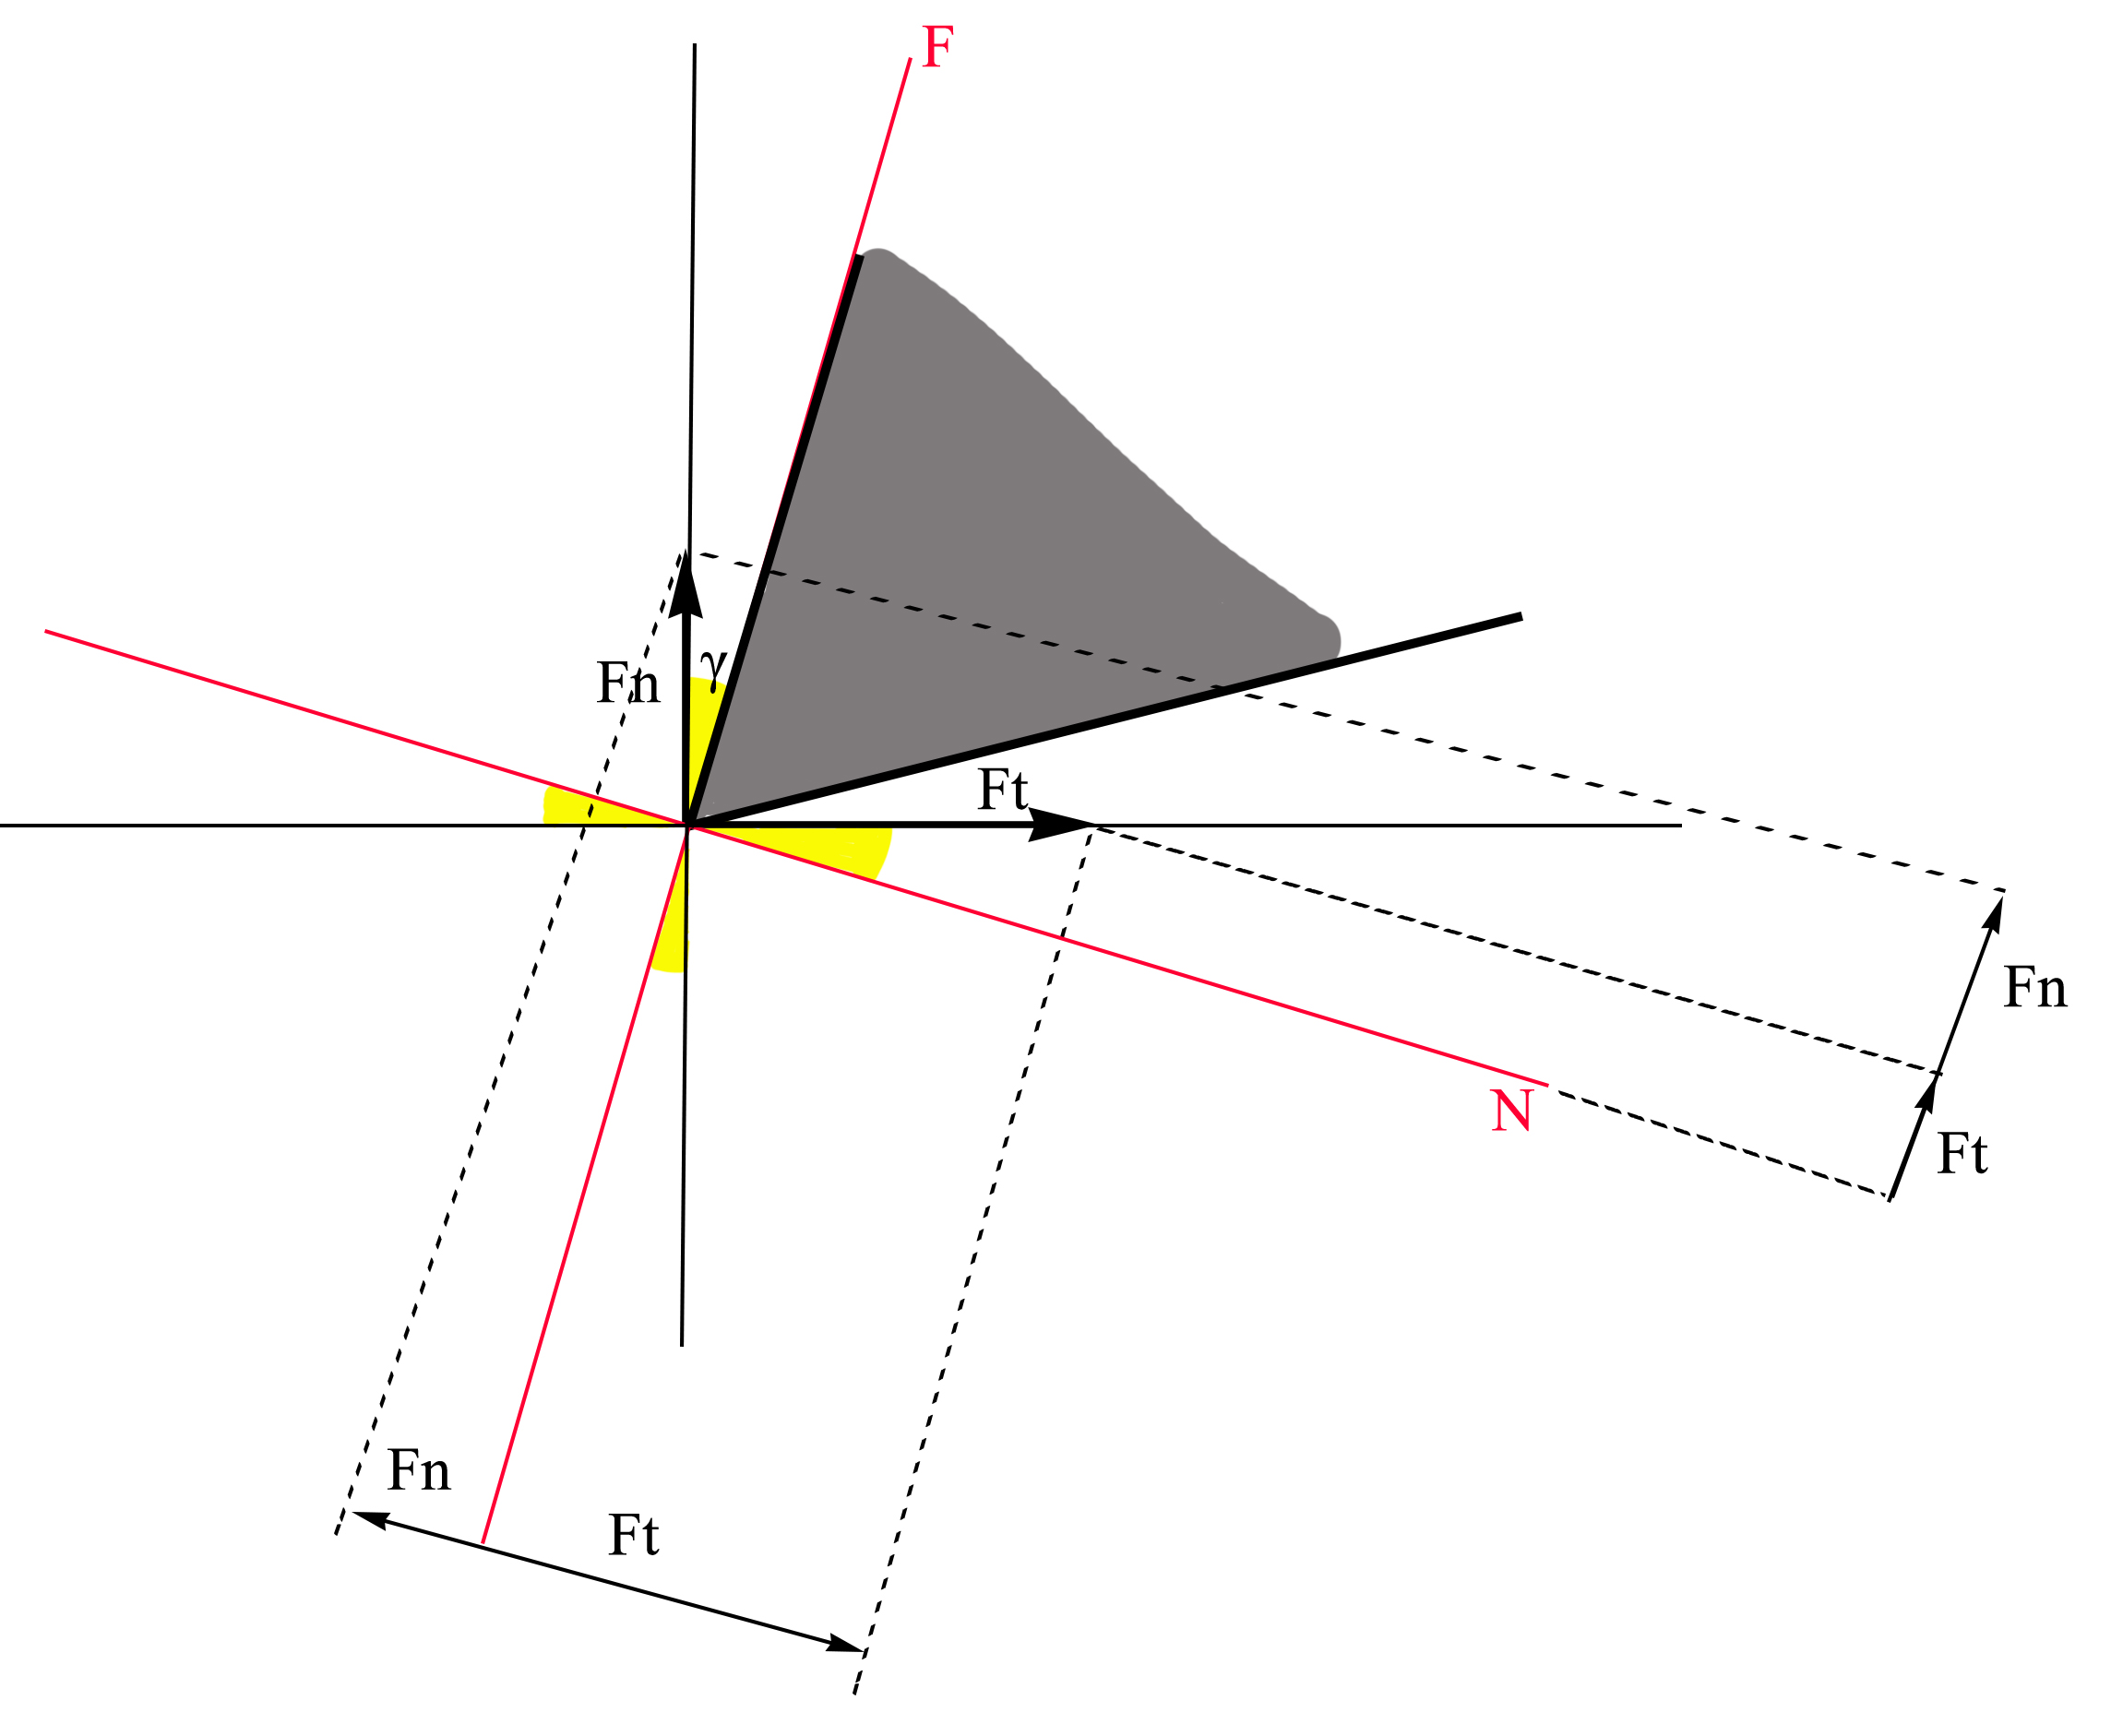
\includegraphics[width=0.5\linewidth]{figures/asp19}
	\end{center}
 	Per cui 
 	\[\begin{cases}
 		N = F_t^N-F_n^N = F_t\cos\gamma-F_n\sin\gamma\\
 		F = F_t^F+F_n^F = F_t\sin\gamma + F_n\cos\gamma
 	\end{cases}\]
	Che conducono a
	\begin{equation}\label{eq:20}
		\boxed{\mu = \tan\rho = {F\over N} = \dfrac{F_t\tan\gamma+F_n}{F_t-F_n\tan\gamma}}
	\end{equation}
\newpage
\section{Usura degli utensili}
\begin{center}
	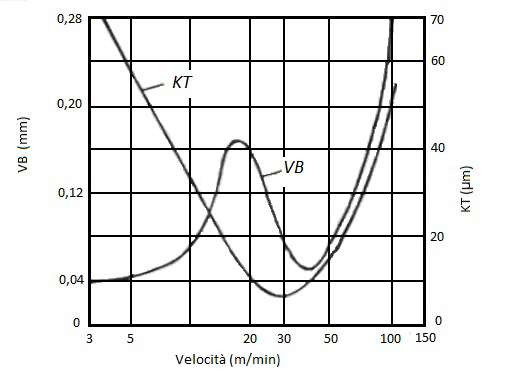
\includegraphics[width=0.7\linewidth]{figures/asp11}
\end{center}
 \begin{table}[H]
 	\begin{tabular}{|c|l|}
 		\hline
 		$v [m/min]$ &
 		\multicolumn{1}{c|}{\begin{tabular}[c]{@{}c@{}}KT\\ Profondità del cratere\end{tabular}} \\ \hline
 		3-30 &
 		\begin{tabular}[c]{@{}l@{}}Decremento con minimo.\\ Formazione del tagliente di riporto che va a proteggere il petto\\ con conseguente strisciamento tra truciolo e tagliente di riporto \\ anziché tra truciolo e petto.\\ Finitura superficiale scarsa.\end{tabular} \\ \hline
 		30-150 &
 		\begin{tabular}[c]{@{}l@{}}Incremento $v\uparrow~T\uparrow$\\ Rimozione del tagliente di riporto.\\ Il petto non è più protetto.\\ Migliore finitura superficiale\end{tabular} \\ \hline
 	\end{tabular}
 \end{table}
 
 \begin{table}[H]
 	\begin{tabular}{|c|l|}
 		\hline
 		$v [m/min]$ &
 		\multicolumn{1}{c|}{\begin{tabular}[c]{@{}c@{}}VB\\ Larghezza del labbro di usura\end{tabular}} \\ \hline
 		3-5 &
 		Andamento costante dato dal tagliente di riporto. \\ \hline
 		5-20 &
 		\begin{tabular}[c]{@{}l@{}}Incremento e massimo.\\ Con $v\uparrow~\gamma\uparrow$\\ Il componente comincia a scaldarsi in corrispondenza \\ del tagliente di riporto.\end{tabular} \\ \hline
 		20-40 &
 		\begin{tabular}[c]{@{}l@{}}Decremento e minimo $v\uparrow~T\uparrow$\\ Il materiale è ora caratterizzato da una bassa $\sigma_y$, \\ le forze in gioco sono minori.\\ Con la $v$ applicata non c'è tempo di formare microsaldature,\\ in più avviene la rimozione del tagliente di riporto\end{tabular} \\ \hline
 		>40 &
 		\begin{tabular}[c]{@{}l@{}}Incremento\\ Oltre a scaldarsi il materiale si scalderà anche l'utensile:\\ anche lui andrà in deformazione plastica. \\ A ciò si aggiunge l'elevato ritorno elastico del materiale di base, \\ questo caratterizzato da un comportamento più rigido\end{tabular} \\ \hline
 	\end{tabular}
 \end{table}
 \newpage
 \section{Calcolo della sezione del truciolo - Tornitura}
\begin{center}
	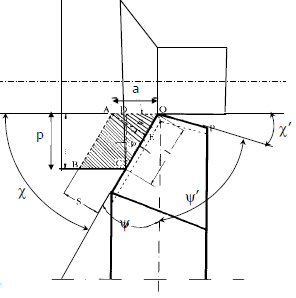
\includegraphics[width=0.3\linewidth]{figures/asp12}
	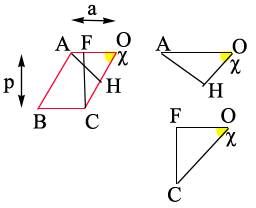
\includegraphics[width=0.3\linewidth]{figures/asp13}
\end{center}
	L'area del parallelepipedo di truciolo vale:
	\[A_{AOCB} = OC\cdot AH = {p\over\sin\chi}\cdot a\sin\chi = a\cdot p\]
	\begin{equation}\label{eq:21}
		\boxed{A = a\cdot p}
	\end{equation}
	In cui $a$ è l'avanzamento e $p$ la profondità di passata.
	\section{Finitura superficiale teorica}
\begin{center}
	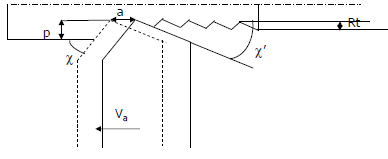
\includegraphics[width=0.5\linewidth]{figures/asp14}
\end{center}	
	Se $\delta={R_t\over2}$ con $R_t$ massima distanza picco-valle in modo che proprio a ${R_t\over2}$ passi la linea di compenso, ovvero la linea media del profilo, è possibile scrivere
\begin{center}
	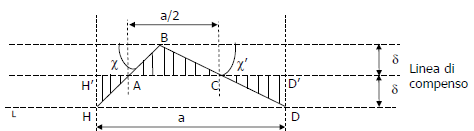
\includegraphics[width=0.7\linewidth]{figures/asp15}
\end{center}
	Per definizione l'entità dello scostamento dal profilo medio è quantificato dalla seguente relazione
	\[R_a = {1\over L}\int_{0}^{L}y(x)dx\]
	Che in questo caso è possibile scrivere come 
	\[R_a = {1\over a} (A_{AHH'} + A_{ABC} + A_{CCD'}) = {1\over a}\left(2\cdot{a\over2}\cdot{\delta\over2}\right) = {\delta\over2} = {R_t\over4}\]
	In definitiva, per profili simmetrici, lineari e ideali il valore di rugosità massimo da aspettarsi è
	\begin{equation}\label{eq:22}
		\boxed{R_t=4R_a}
	\end{equation} 
	\newpage
	\begin{center}
		{\small\textit{Non c'è sulle slide, però magari può servire...}}
	\end{center}
	È possibile mettere in relazione $R_a$ con gli angoli di registrazione del tagliente primario $\chi$ e del tagliente secondario $\chi'$
\begin{center}
	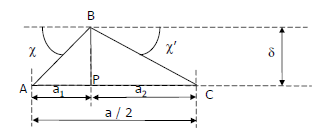
\includegraphics[width=0.7\linewidth]{figures/asp16}
\end{center}
	\[{a\over2} = a_1 + a_2\]
	Ma
	\[\delta = a_1\tan\chi = a_2\tan\chi'
	 \Rightarrow \begin{cases}
	a_1 = \dfrac{\delta}{\tan\chi} \\
	a_2 = \dfrac{\delta}{\tan\chi'}
	\end{cases}\]
	E quindi
	\[{a\over2} = \delta\left(\dfrac{1}{\tan\chi} + \dfrac{1}{\tan\chi'}\right)\]
	Per cui, risolvendo per $\delta$ si ottiene 
	\[\delta = \dfrac{\nicefrac{a}{2}}{\dfrac{1}{\tan\chi} + \dfrac{1}{\tan\chi'}}\]
	E quindi
	\[R_a = {\delta\over2} = \dfrac{\nicefrac{a}{4}}{\dfrac{1}{\tan\chi} + \dfrac{1}{\tan\chi'}}\]
	Per cui come $\chi, \chi', a$ aumentano aumenta $R_a$
	\newpage
	\section{Finitura superficiale reale}
	Nella realtà un utensile non può essere perfettamente affilato perché significherebbe non avere alcuna sezione resistente, all'applicazione del carico andrebbe subito in deformazione plastica.
	
	Nella realtà l'utensile è raccordato. 
\begin{center}
	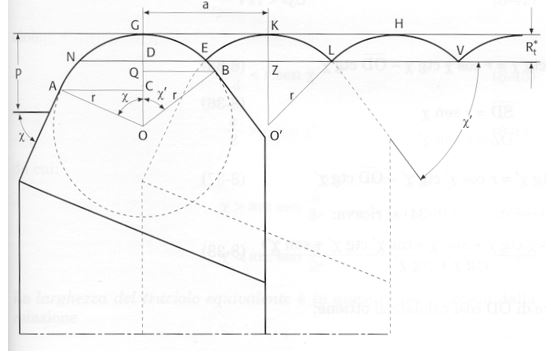
\includegraphics[width=0.7\linewidth]{figures/asp17}
\end{center}
	Si zoomma sul profilo del pezzo, si traccia un'orizzontale passante per tutte le valli del profilo: $N, E, L, V$; dopodichè si tracciano i raggi di curvatura come segmenti perpendicolari all'orizzontale: $GO$ e si determinano i segmenti $ND$ e $DE$. 
	
	Si individuano poi i punti $A$ (risp. $B$) punti di tangenza tra il cerchio osculatore in $G$ ed il tagliente principale (risp. secondario), a questo punto possono essere tracciati i segmenti $AC$ e $QB$. \\
	
	Quindi le condizioni da rispettare sono
	\[ND<AC\qquad DE<QB\]
	In parole, il raggio di raccordo che sta partecipando alla generazione del profilo sia minore del raggio di curvatura del tagliente principale/secondario. 
	
	Ciò si può facilmente riscrivere come 
	\[{a\over2}<r\sin\chi\qquad{a\over2}<r\sin\chi'\]
	Per cui affinché la generazione del profilo avvenga interessando esclusivamente il
	raggio di raccordo dovranno essere verificate le seguenti condizioni
	\[\begin{cases}
		\chi>\arcsin\left(a\over2r\right)\\
		\chi'>\arcsin\left(a\over2r\right)
	\end{cases}\]
	\newpage
	La massima rugosità ottenibile da quel raggio di raccordo si ottiene osservando che
	\[R_t = GD = OG - OD = \left(r-\sqrt{r^2-{a\over4}}\right)\cdot10^3\qquad\mu m\]
	Se secondo Schamlz è possibile approssimare l'arco di circonferenza $NE$ ad un arco di parabola, è possibile scrivere 
	\[R_t^* = {a\over8r}10^3\qquad\mu m\]
	E quindi 
	\begin{equation}\label{eq:23}
		\boxed{R_a^* = {R_t^*\over4} = {a^2\over23r}10^3\qquad\mu m}
	\end{equation}
	 \section{Calcolo della sezione del truciolo - Foratura}
\begin{center}
	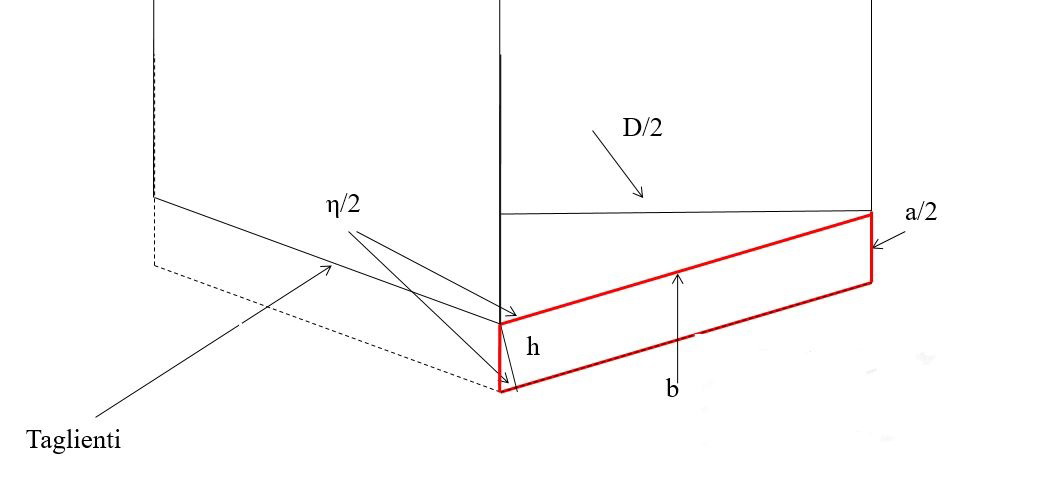
\includegraphics[width=0.7\linewidth]{figures/asp18}
\end{center}
	L'area del generico parallelepipedo vale 
	\[A = b\cdot h\]
	In cui
	\[b = {D\over2}\cdot\dfrac{1}{\sin{\eta\over2}}\qquad h = {a\over2}\cdot\sin{\eta\over2}\]
	E allora 
	\[A = {D\over2}\cdot{a\over2} = \dfrac{Da}{4} \]
	
	
\newpage	
	
	
\part{Frequently Asked Questions}

\begin{itemize}
	
\item \textcolor{red}{\textbf{Per quale motivo al variare di $\gamma$, e quindi aumentando $\gamma$, si ha una riduzione della deformazione plastica?}}\\
%\begin{enumerate}
%	\item \textit{Perché secondo Pijspanen $2\phi-\gamma = {\pi\over2}$ e aumentando $\gamma$ deve per forza aumentare anche $\phi$, e quindi diminuirà la deformazione plastica}
%	\item \textit{Avere un $\gamma$ elevato porta ad avere un utensile più affilato e quindi effettuare più facilmente il taglio, questo perché la dimensione del tratto $OA$ è minore e ci sono meno atomi da spostare per completare il lavoro}
%\end{enumerate}

\item
\textcolor{red}{\textbf{Perché sono stati introdotti i metodi di Pijspnanen e di Merchant e su quali basi? Quali sono le loro differenze?}}\\
%\textit{Il modello di Pijspanen si prefigge il compito di relazionare l'angolo di spoglia superiore
%dell'utensile a quello di scorrimento del materiale interessato, questo per far si che avvenga la deformazione plastica.
%	Considera il materiale come composto da tante lamelle e l'avanzamento dell'utensile sospinge ciascun elemento in avanti 
%	obbligandolo a scorrere sull'elemento successivo.
%	La forza che l'utensile applica sul truciolo dev'essere in grado di generare sul piano di scorrimento
%	una tensione tangenziale necessaria e sufficiente a provocare lo scorrimento delle lamelle.
%	Il modello di Pijspanen si basa sull'esistenza di un unico piano di scorrimento, ipotesi in prima approssimazione 
%	avvalorata dato che l'estensione della zona di scorrimento tende a un unico piano per i valori delle velocità di taglio comunemente impiegati.}
%[DIMOSTRAZIONE]
%
%\textit{Il modello di Merchant viene studiato per quantificare le forze in gioco nel processo di taglio. 
%	Se si considera il truciolo come un corpo libero, questo, istante per istante, dovrà essere in equilibrio sotto l'azione delle forze 
%	applicate dall'utensile e quelle di resistenza sviluppate dal materiale.
%	Il modello di Merchant prevede di inscrivere, proiettando, tutte le forze in gioco nell'asportazione di materiale all'interno di una circonferenza 
%	tangente al tagliente avente come diametro il modulo della risultante delle forze, questa uguale per tagliente e truciolo.
%	È ora necessario eseguire una distinzione tra i due modelli proposti da Merchant. 
%	Nel primo modello si avrà deformazione plastica del truciolo, e quindi taglio, appena sul piano di scorrimento si raggiunge la \textbf{tensione dinamica di scorrimento} $\tau_s$.}
%[DIMOSTRAZIONE]
%\textit{Il secondo modello viene proposto perchè il primo entra in discordanza coi dati sperimentali, questa discordanza è dovuta proprio alla tensione tangenziale $\tau_s$ necessaria a 
%	provocare lo scorrimento, che non è una quantità costante ma funzione della tensione normale che agisce sul medesimo piano di scorrimento, secondo la relazione
%	\[\tau_s = \tau_{s0}+K\sigma_s\]
%	Nel suo primo modello Merchant considera $\tau_s$ come costante, ma nel momento in cui si ha una componente normale al piano di scorrimento, 
%	questa avvicina gli atomi tra loro e conseguentemente ciò comporta un aumento della tensione di taglio necessaria allo scorrimento: le celle 
%	elementari vengono compresse e il parametro di cella $a$ diminuisce, con $b$ distanza tra gli atomi sul piano di scorrimento.}
%[RISULTATO/DIMOSTRAZIONE]

\item
\textcolor{red}{\textbf{Fattore di ricalcamento}}\\
%\textit{La deformazione plastica del materiale avviene per scorrimento e l'angolo di scorrimento $\phi$ individua il piano di scorrimento; 
%	questo è calcolabile conoscendo altezza di passata $s$ e l'altezza del truciolo $s_1$. 	
%	Si definisce il fattore di ricalcamento $c$:
%	\[c = {s\over s_1}\]
%	Si può ricavare attraverso il fattore di ricalcamento il valore di $\phi$ conoscendo $\gamma$}
%[DIMOSTRAZIONE]





\item
\textcolor{red}{\textbf{Per quali motivi perché vengono effettuate le lavorazioni per asportazione di truciolo?}}\\
%\textit{Si fanno per ottenere un parametro di rugosità migliore, un fattore di finitura superficiale maggiore rispetto alle altre lavorazioni. 
%	Permette di ottenere un prodotto finito, che può essere già venduto, a differenza del processo di fonderia.}





\item
\textcolor{red}{\textbf{Come si fa a capire quale sia il processo migliore per la lavorazione di un prodotto tra asportazione del materiale, processo di fonderia e deformazione platica?}}\\
%\textit{Le potenze in gioco sono nettamente differenti. 
%	Se il lotto è numeroso si predilige un processo in fonderia, magari in forma permanente, con successiva defromazione plastica e trattamenti termici (normalizzazione, rinvenimento, tempra), altrimenti, se il lotto non è numeroso
%	è possibile anche affettuare un processo fusorio in forma transitoria con successiva o defromazione plastica o asportazione di truciolo.
%	Per la produzione di un solo pezzo in particolare è preferibile l'asportazione di materiale perchè se si volesse defromare plasticamente quel singolo pezzo  si necessiterebbe di un solo
%	stampo che costa molto, ed è economicamente sconveniente.
%	In più, per materiale che devono, per loro condizioni d'impiego, ad esempio resistere a carichi di fatica, è preferibile lavorare per fonderia in forma permanente e asportazione di materiale,
%	la prima consente di avere un controllo maggiore sulla micrografia del componente, mentre la seconda garantisce miglior finitura superficiale e minori probabilità di fornire inneschi di cricche.}




\item
\textcolor{red}{\textbf{Fiamma Ossacetilenica}}\\
%Pericolo per saldatura di fiamma ossiacetilenica :
%Praticità operatore,
%Le t sono basse
%Non posso saldare tutti i materiali 
%Se voglio saldare un materiale con uno spessore maggiore faccio un movimento a spingere.





\item
\textcolor{red}{\textbf{Slab Metod e Trafilatura}}\\
%si fa sopratutto a freddo perché se a caldo, avrei materiale meno duttile e non avrei più incrudimento se fosse a caldo.
%Permette di applicare un equilibrio ad un pezzo interno per valutare le forze.
%Come faccio a collegare questo stato triassale con lo slab metod?
%Uso von mises per passare per passare da uno stato tridimensionale ad uno stato piano.
%Usando Sachs ho sigma1+sigma2=sigma0





\item
\textcolor{red}{\textbf{Perché non avviene un incrudimento nelle lavorazioni a caldo?}}\\
%Siamo di solito al 60 per cento della t di fusione,
%Si ha incrudimento quando le deformazioni si impilano e viene meno il primo moto.
%Dimostrazione come si muovono le dislocazioni nella deformazione plastica 
%Quando si ha una dislocazione si muove la dislocazione e non gli atomi perché la tensione critica è proporzionale a b distanza tra gli atomi.





\item
\textcolor{red}{\textbf{Da cosa deriva una rugosità in una lavorazione di tornitura?}}\\
%	Dipende dal raggio dell utensile 
%	Il raggio di raccordo non è il tagliente principale 
%	Non è la Rugosità teorica il Rt perché questa è quella che si ottiene dall approssimazione ma non è detto che è quella che realmente otteniamo. Rt e la distanza picco valle. Abbiamo definito Rt teorica perche si è fatta un approsimazuone geometrica come se è fatto una sezione perché ho considerato i punti per avanzamenti successivi. E teorico perché è ipotetico ad un cinema stimo del mio utensile e non è un profilo perfettamente calcolato.
%	Ra rappresenta lo scostamento dalla linea media
	
	
	
	
	
\item
	\textcolor{red}{\textbf{A cosa serve la durezza e le sue prove?}}\\
%	Sono prove non distruttive, sono necessaire solo quando ho bisogno di prestazioni esterne. 
%	La durezza è importante per utensili che si usurano, da una informazione adeguata riguardo alla resistenza all usura. Misura L impronta lasciata dal materiale, sorta di deformazione plastica.
%	Differenza prova di trazione, prova qualsiasi, e durezza
%	Vengono eliminati ossidi e contaminanti nelle prove di durezza visto che si riferisce all esterno. Il comportamento di un materiale su una sup è diversa ed è dovuto dalla struttura del materiale
	
	
	
	
\item
	\textcolor{red}{\textbf{Si può notare il carattere di durezza del materiale anche dal diagramma tensione deformazione $\sigma\varepsilon$?}}\\
		
		
		
		
		
		
\item
		\textcolor{red}{\textbf{Come ottenere dei grani colonnari?}}\\
%		Differenza temperatura processo fusorio
%		I grani colonnari crescono in questo modo  perché è legato alla temperatura
%		Cos è il gradiente termico
		
		
		
		
		
\item
		\textcolor{red}{\textbf{Differenze tra forma permanente e transitoria. Quali sono i loro vantaggi?}}\\
%		Sabbia silicea e argilla fatta da legante sono formate le terre.
%		Le forme permanenti devono avere una geometria semplice per il problema dell estrazione perché deve garantire un metodo di estrazione che non possa rovinare lo stampo.
%		Forma transitoria si estrae il modello ecco perché possiamo avere forme più complicate.
%		Le differenze tra le dimensioni degli stampi utilizzati per i due processi sono dovuti 
%		Non sono vincolati per agevolare L operatore di avere piccole forme nella forma transitoria.
%		Mentre per la forma permanente le dimensioni del componente sono vincolate per limiatare il fatto che si hanno in gioco forze e pressioni molto elevate.
%		Attraverso L applicazione di pressione riduco il tempo ciclo, garantire che la cavità sia completamente riempita prima che inizia la solidificazione, per evitare il problema della contropressione ma sopratutto perché si riducono i tempi di solidificazione perché la pressione spinge le molecole tra loro che le costringe a legarsi e a formare dei legami molecolari prima tra loro.
%		Non essendo poroso il metallo.
		
		
		
		
		
\item
		\textcolor{red}{\textbf{Differenze tra processo fusorio di un metallo puro e di una lega}}\\
%		La fine solidificazione di tutto il materiale avviene li perché deve aspettare che si solidifichi il materiale basso fondente.
%		Si formano dendriti dovute al fatto che il materiale altofondente rispetto a quello basso fondente si solidifica prima.
%		Le dendriti hanno un ramo secondario e uno principale 
%		Posso evitare le dendriti se gli elementi di leghe hanno le stesse o simili T oppure evitando di far muovere gli atomi cercando di bloccarli e quindi devo raffreddare molto velocemente i materiali. Questi problemi si hanno per le forme transitorie.
		
		
		
		
		
\item
		\textcolor{red}{\textbf{Attrito adesivo}}\\
%		Ci permette di fare la lavorazione di laminazione. Si hanno attriti come quello cououmbiano o quello della torria adesiva visto perché il primo non ci permette di capire perché al variare della t il coefficiente di attrito aumenta.
%		Ecco perché abbiamo introdotto la teoria adesiva.
%		Il coefficiente di attrito adesivo rappresenta la forza tangenziale che dobbiamo applicare per
%		dipende dal materiale stesso
		
		
		
		
		
\item
		\textcolor{red}{\textbf{Condizioni di imbocco spontaneo per la laminazione,  quando queste non sono verificate come posso garantire la laminazione continua?}}\\
%			Si ha imbocco spontaneo se la forza tangenziale maggiore di quella radiale.
%			A freddo ho più controllo sulla rifinitura mentre a caldo ho i problemi di ossidi.
			
			
			
			
			
\item
			\textcolor{red}{\textbf{Difetti di laminazione}}\\
%				La fibra all esterno sarà più corta nel processo di laminazione ovvero quella andata a contatto con il rullo rispetto a quella centrale perché c’è L attrito che tende a fermare la velocità.
				
				
				
				
				
\item
				\textcolor{red}{\textbf{Differenze nella lavorazione di tornitura}}\\
					
					
					
					
					
\item
					\textcolor{red}{\textbf{Parametri che influenzano l'asportazione di materiale}}\\
%						sono profondità di passata avanzamento e la velocità di taglio 
						
						
						
						
						
\item
\textcolor{red}{\textbf{Usura degli utensili. Perché il massimo di VB e il minimo di KT non coincidono?}}\\
%(GRAFICO E TABELLA)
%Perché ad una velocità di circa 20 metri/minuto inizia ad esserci il distacco del tagliente di riporto e ciò comporta una profondità del cratere crescente: ci sono delle forze d'attrito 
%che all'avvinarsi di quella velocità fanno si che ci sia usura adesiva in corrispondenza del tagliente. 
%Inoltre aumentando la velocità aumenta si la temperatura e quindi si è portati a credere che sia più preponderante il fenomeno dell'adesione, tuttavia questo viene meno perché non c'è 
%il tempo necessario affinché il truciolo possa effettivamente diffondere e microsaldarsi al tagliente. 

\item 
\textcolor{red}{\textbf{Stampaggio e relativo grafico}}\\

\item 
\textcolor{red}{\textbf{Differenze e scelte di materiale per comportamento a creep e a fatica}}\\		

\item 
\textcolor{red}{\textbf{Tempo di lavoro ed MRR}}\\	

\item 
\textcolor{red}{\textbf{Prepararsi un argomento a piacere}}\\							
							
			
\end{itemize}				

\end{document}